% !TeX program  = XeLaTeX
% !TeX encoding = UTF-8
\documentclass[a4paper]{nuist}


\usepackage{tikz}
\usepackage{extarrows}
\usepackage[thicklines]{cancel}
\usepackage{subfigure}
\usetikzlibrary{plotmarks}
\usepackage{pgfplots}
\title{扩散与逆扩散过程的总览、原理与推导}
\author{
    周肖桐 \\
}
\date{\today}
\begin{document}

\cover{基于扩散的图像生成模型与DDPM原理}
{周肖桐}{202312200030}{计算机学院、\\网络空间安全学院}{计算机技术}{余文斌}{二O二四\hspace{0.4em} 年\hspace{0.4em} 六\hspace{0.4em} 月\hspace{0.4em} 二十一\hspace{0.4em} 日}

\tableofcontents
\newpage


% \begin{equation}
%   \begin{aligned}
%       P_\theta(x_i)\\
%       x_1,x_2, \cdots, x_n\\
%       \vec{\theta}\\
%       \prod_{i=1}^{n} P_\theta (x_i)\\
%       \vec{\theta^*} =  \text{avg} \max \prod_{i=1}^{n} P_\theta (x_i)
%   \end{aligned}
% \end{equation}

% \begin{tikzpicture}
%   \begin{axis}[
%     xlabel=$x$,
%     ylabel=$P(x)$,
%     domain=-3:3,
%     samples=100,
%     smooth,
%     no markers,
%     axis lines=center,
%     x axis line style={->},
%     y axis line style={-},
%     ]

%     \addplot {exp(-x^2/2)/sqrt(2*pi)};

%     % 画两条竖线
%     \draw[dashed] (axis cs: 0, 0) -- (axis cs: 0, {exp(0)/sqrt(2*pi)});
%     \draw[dashed] (axis cs: 1, 0) -- (axis cs: 1, {exp(-1)/sqrt(2*pi)});

%     % 在两条竖线之间添加阴影
%     \fill[gray!20, domain=0:1]
%     (axis cs: -0.2, 0.5) -- % 使用 exp(0) 代替 exp(-0^2/2),即 x=0 处的值
%     (axis cs: -0.2, 0) -- (axis cs: 0.2, 0) -- (axis cs: 0.2, 0.5) -- cycle;

%   \end{axis}
% \end{tikzpicture}

% \begin{tikzpicture}
%   \begin{axis}[
%     xlabel=$x$,
%     ylabel=$P(x)$,
%     domain=-4:4,
%     samples=100,
%     smooth,
%     no markers,
%     axis lines=center,
%     x axis line style={->},
%     y axis line style={->}
%     ]
    
    
  
%     \addplot[fill=gray!20, draw=none, domain=-0.2:0.2, samples=50] {exp(-x^2/2)/sqrt(2*pi)} \closedcycle;
  
%   % 画两条竖线
%       \draw[dashed] (axis cs: -0.2, -0.1) -- (axis cs: -0.2, {exp(-0.04)/sqrt(2*pi)});
%       \draw[dashed] (axis cs: 0.2, -0.1) -- (axis cs: 0.2, {exp(-0.04)/sqrt(2*pi)});
%       \addplot {exp(-x^2/2)/sqrt(2*pi)};
%       \node at (axis cs: -0.52, 0.018) {$x_2$};
%       \node at (axis cs: 0.52, 0.018) {$x_2$};
%     \end{axis}
% \end{tikzpicture}


%\newpage

\section*{摘要}

本文介绍了风格迁移的由来以及分类。
\maketitleofchinese{基于扩散的图像生成模型与DDPM原理}{周肖桐\footnote{E-mail:\url{xiaotongzhounuist@163.com}}}{计算机学院、网络空间安全}

\abstractofchinese{本文旨在全面概述和深入分析扩散与逆扩散过程在图像生成模型中的应用与理论基础。文章分为三个主要部分:首先总览扩散模型的图像生成过程, 并作为扩散与逆扩散过程的引入。其次,详细阐述扩散过程与逆扩散过程的概念与区别,讨论这些过程在图像生成中的重要性及其工作原理。最后,通过数学公式推导,深入解析扩散与逆扩散过程的具体实现,提供系统性的理论支撑,并对其性能和有效性进行评估。本文通过对这两种过程的全面分析与推导,旨在为图像生成领域的研究者提供有价值的参考与指导。}{扩散模型、原理介绍、公式推导}


\maketitleofenglish{Diffusion Based Generation Model \& Principles of DDPM}{Xiaotong Zhou\footnote{E-mail: \url{xiaotongzhounuist@163.com}}}{School of Computer Science}

\abstractofenglish{This paper aims to provide a comprehensive overview and in-depth analysis of the application and theoretical foundation of diffusion and reverse diffusion processes in image generation models. The article is divided into three main sections: First, it introduces the basic image generating process of DDPM, aiming to explore the structural similarities of these models and to serve as an introduction to diffusion and its reverse processes. Second, it elaborates on the concepts and differences between the diffusion process and the reverse diffusion process, discussing their importance and working principles in image generation. Finally, through mathematical formula derivation, it delves into the specific implementation of diffusion and reverse diffusion processes, providing systematic theoretical support and evaluating their performance and effectiveness. By providing a comprehensive analysis and derivation of these two processes, this paper aims to offer valuable reference and guidance for researchers in the field of image generation.}
{Diffusion models, Principles introduction, Formula derivation}


\section{简介}

风格迁移是一种计算机视觉和图像处理领域的技术,它旨在将一幅图像的艺术风格应用于另一幅图像,从而创造出全新的图像。这一技术的应用非常广泛,从艺术创作到图像编辑都有涉及。风格迁移有两种主要方法:传统方法和基于神经网络的方法。

传统方法通常使用数学和信号处理技术,如纹理合成、直方图匹配和滤波等。这些方法涉及对图像的像素进行操作,以模拟所需的风格。例如,可以通过频域滤波来增强或减弱图像的某些频率成分,从而改变其外观。传统方法的好处在于它们通常计算速度较快,但它们可能无法捕捉到更高级的艺术风格和纹理。

基于神经网络的风格迁移方法则更加先进和强大。这些方法使用深度学习技术,来学习和应用图像的风格。它们通过训练神经网络来捕捉不同艺术风格的特征,然后将这些特征应用于输入图像,以生成具有所需风格的新图像。这种方法的好处在于它能够更好地捕捉到艺术风格的细节和复杂性,计算成本随使用的模型的差别而有所差别。

传统的风格迁移方法与基于神经网络的风格迁移方法之间并不应该事被代替与代替的关系,相反,目前许多基于神经网络的风格迁移方法的思想来源于传统的风格迁移方法。同时,基于神经网络的风格迁移技术也有一些缺陷,如伪影、难以控制风格化过程等缺陷,将传统风格迁移与基于神经网络的风格迁移工作相结合反而可能会取得更好的结果。

风格迁移技术的应用领域广泛,包括图像风格化、电影特效、艺术创作和图像编辑。无论是传统方法还是基于神经网络的方法,风格迁移都为图像处理提供了强大的工具,可以创建出富有艺术感和创新性的图像。


\section{写在开始前}

在开始前,我想先解释一下本文中两个名词『DDPM』与『基于扩散的图像生成模型』之间的差异,以解释本文内容与标题之间的联系。
本文中的『DDPM』指的是文章Denoising Diffusion Probabilistic Model\cite{hoDenoisingDiffusionProbabilistic2020a}中提出的模型,是最早的『基于扩散的图像生成模型』。
而『基于扩散的图像生成模型』指的是以所有扩散过程与逆扩散过程作为基本原理的图像生成模型。
本文的标题为『基于扩散的图像生成模型与DDPM原理』,实际上是在介绍两个部分,其一为『基于扩散的图像生成模型』,其二为『DDPM原理』。第一部分将接受当前所有的『基于扩散的图像生成模型』的总体工作流程,从整体的角度为各位介绍该类模型的生成过程。第二部分以最简单的『基于扩散的图像生成模型』,也即DDPM作为基础,为各位推导最简单的流程。

下面开始第一部分,介绍『基于扩散的图像生成模型』的基本流程。

\section{基于扩散的图像生成模型的基本流程}

该部分介绍基于扩散的图像生成模型的基本工作流程,为不了解该类模型的读者简单介绍一下模型的生成过程,为后面详细介绍原理做准备。

首先需要明确的是『扩散过程与逆扩散过程』与『基于扩散的图像生成模型』这两个名词之间的差别。有些文章可能将这两个概念混淆,或直接称『基于扩散的图像生成模型』为『扩散模型』,但本文希望能将这两个概念进行辨析,以获得更明确无歧义的阅读体验。

『扩散过程与逆扩散过程』可以分成两个过程,即『扩散过程』与『逆扩散过程』。『扩散过程』其实是一个物理过程,图像生成模型中模仿这个概念,让噪声逐渐扩散到整个图像的过程被称为『扩散过程』;而『逆扩散过程』则是将扩散过程反过来,从噪声图像中恢复出一张不带有噪声的图像的过程。扩散过程可以看作『基于扩散的图像生成模型』中的一个基本原理。

而『基于扩散的图像生成模型』则是以『扩散过程与逆扩散过程』作为基本原理,进行图像生成的模型,二者是包含与被包含的关系。后者包含前者,而前者作为后者的一部分,为后者提供服务。本文中对于『扩散过程与逆扩散过程』与『基于扩散的图像生成模型』这两个概念均与上述描述保持一致,若在阅读中出现概念对这两个概念混淆的现象,可以翻阅本段文字或查阅\ref{sec_noun}名词解释部分作为参考。

其次需要介绍的是『基于扩散的图像生成模型』的输入与输出。该类模型接收对于图像的文字描述作为输入,并输出一张或多张与输入文字描述相符合的图像,如下图\ref{fig_ioput_of_model}所示。

\begin{figure}[htbp]
    \centering
    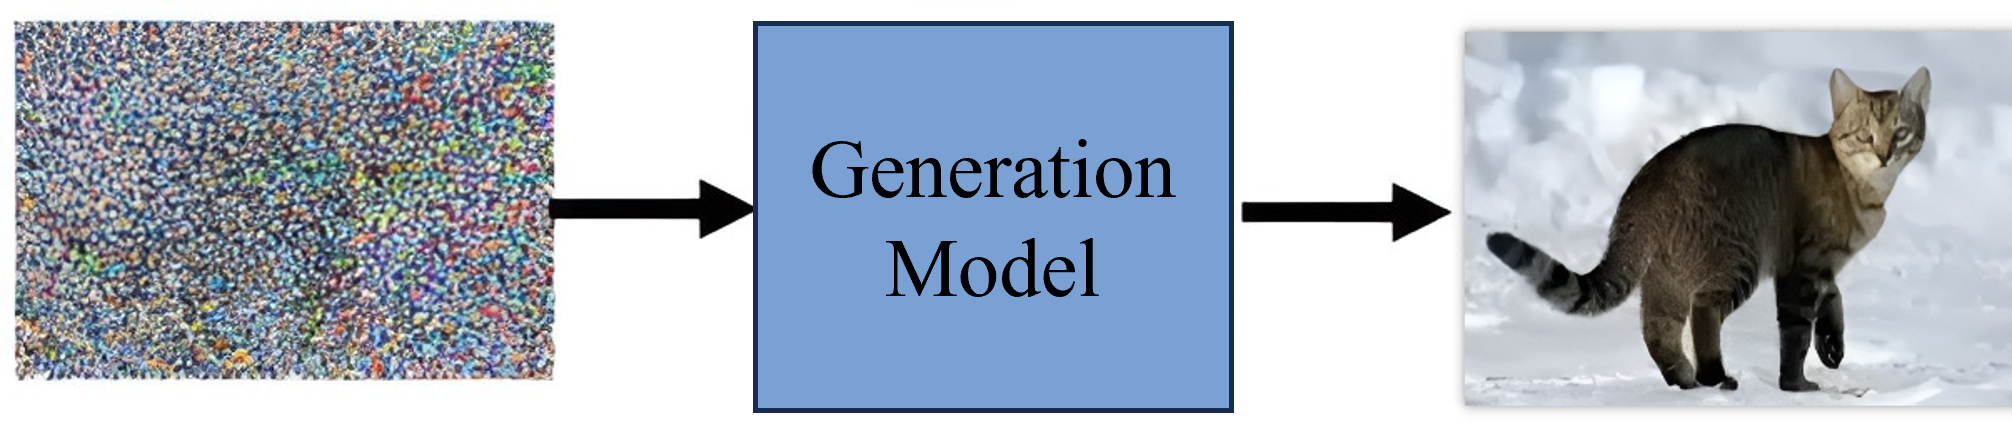
\includegraphics[width=0.8\textwidth]{figs/color/ioput_of_model.png}
    \caption{基于扩散的图像生成模型:输入与输出}
    \label{fig_ioput_of_model}
\end{figure}

当接收到文字输入后,『基于扩散的图像生成模型』将随机从高斯分布中采样一张噪声图像,并将该噪声图像与文字输入一同送进Denoise模块中。Denoise模块将去除噪声图像中的部分噪声,从而得到一张部分降噪的图像。这个过程如下图\ref{fig_denoise}所示。

\begin{figure}[htbp]
    \centering
    \subfigure[Denoise模块的输入与输出]{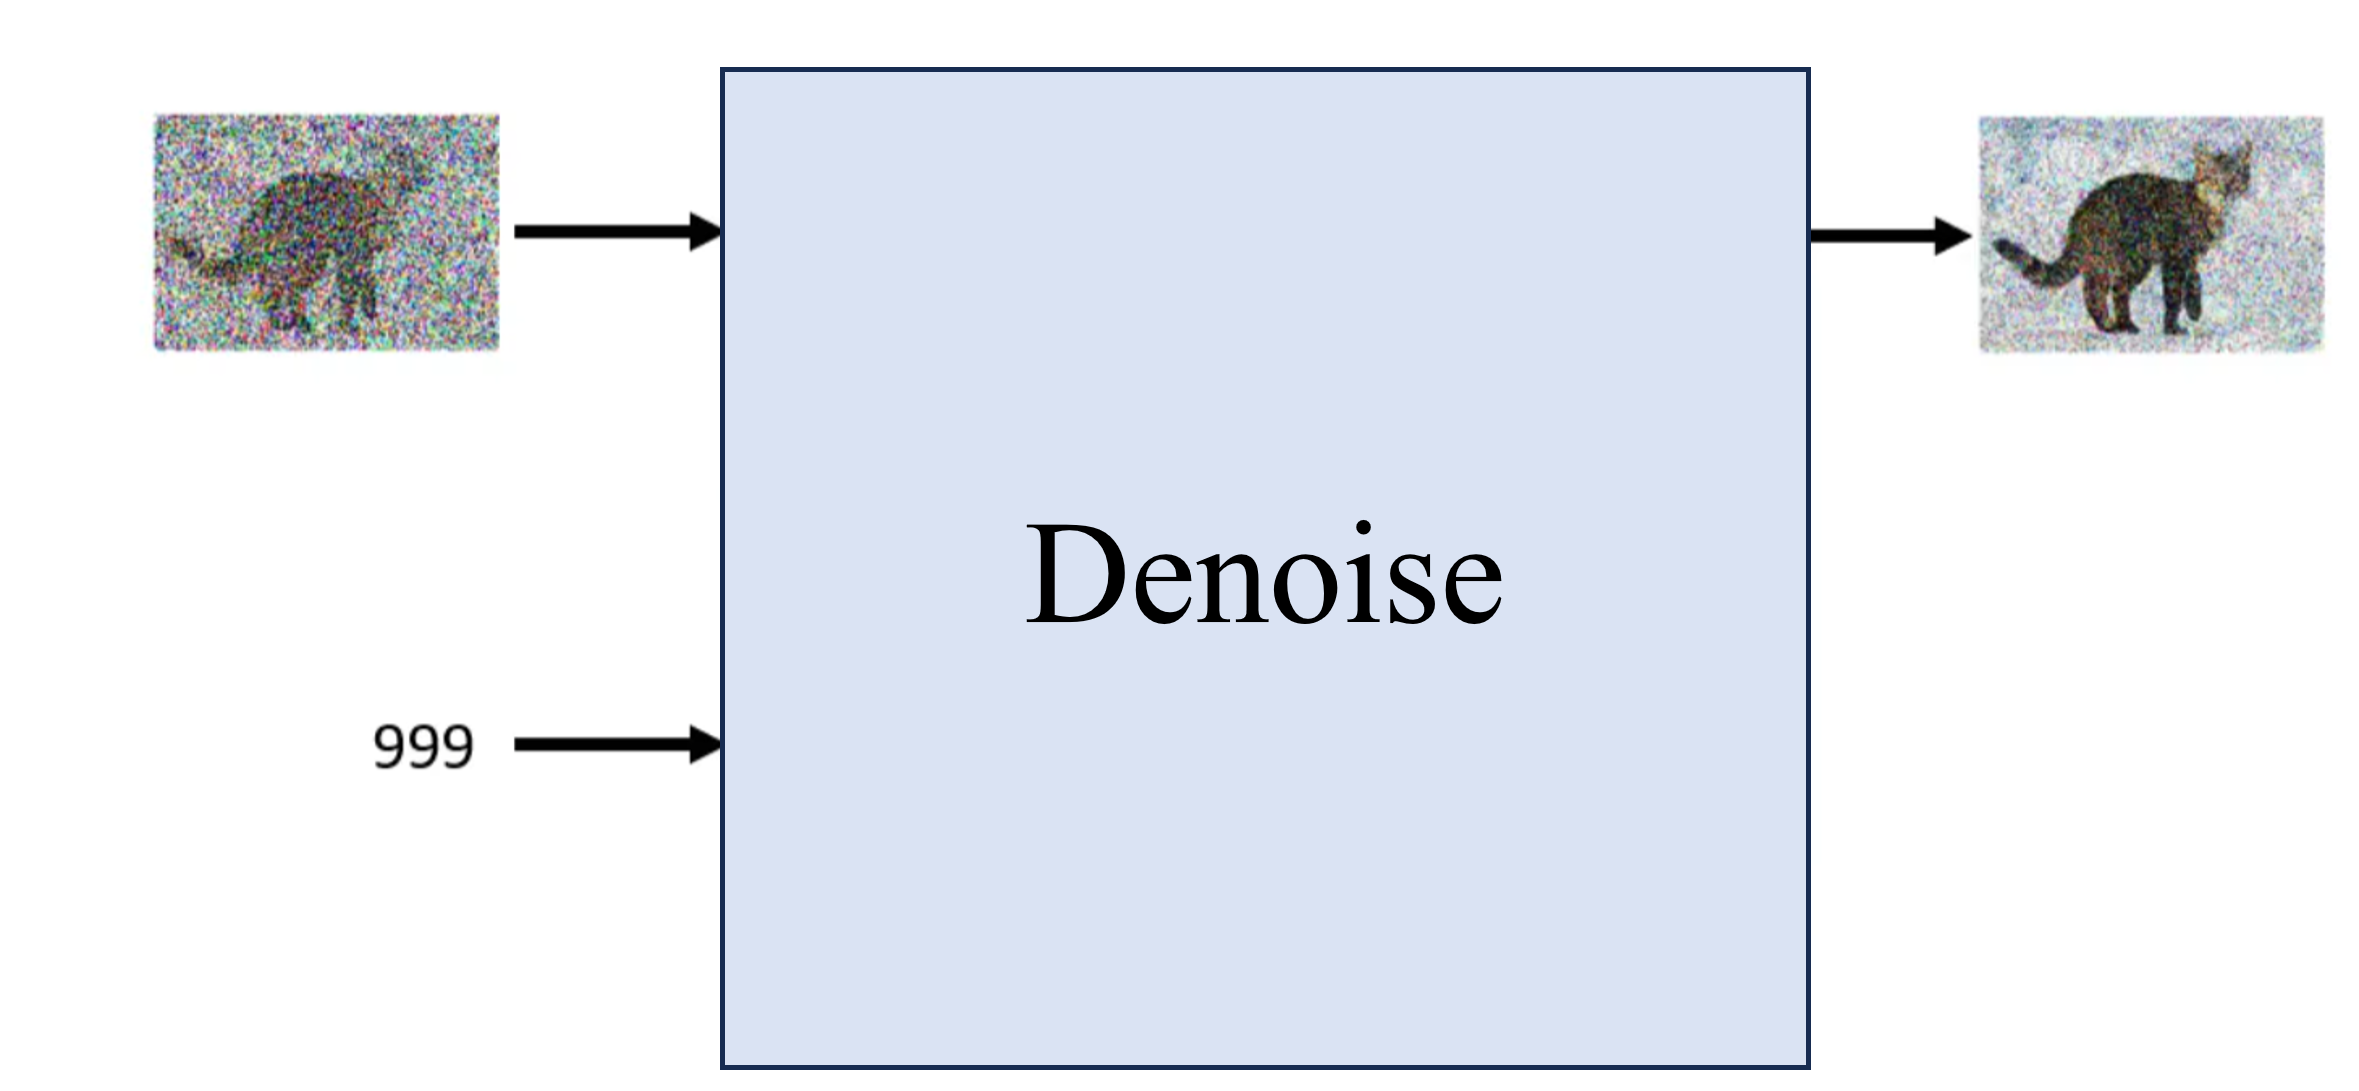
\includegraphics[width=0.4\textwidth]{figs/color/denoise.png}}
    \subfigure[单个Denoise过程]{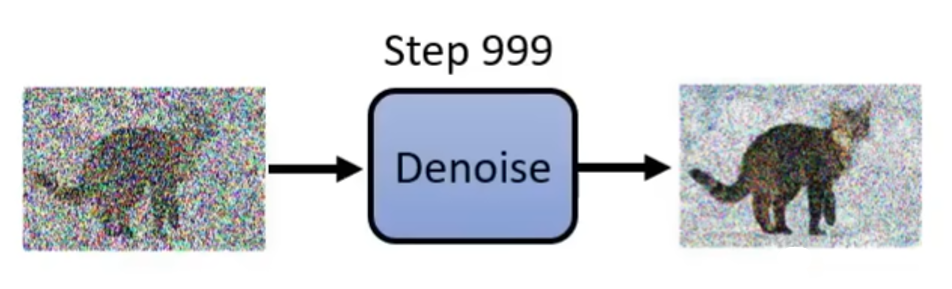
\includegraphics[width=0.4\textwidth]{figs/color/denoise1.png}}
    \caption{基于扩散的图像生成模型:Denoise模块}
    \label{fig_denoise}
\end{figure}


将得到的部分降噪图像重新输入到Denoise模块中,重复多次,便可得到一张符合输入文字描述的图像。这就是『基于扩散的图像生成模型』的基本工作流程,如图\ref{fig_process_of_model}所示。

\begin{figure}[htbp]
    \centering
    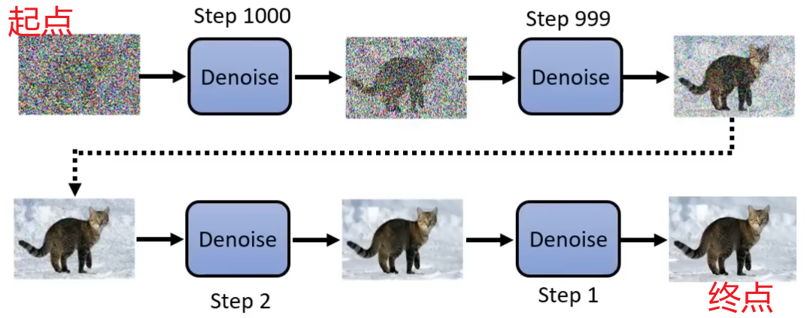
\includegraphics[width=0.8\textwidth]{figs/color/process.png}
    \caption{基于扩散的图像生成模型:整体工作流程。用一句话概括上述对『基于扩散的图像生成模型』工作流程的描述:『基于扩散的图像生成模型』接收对于图像的描述作为输入,对自己生成的一张噪声图经过多次去噪操作后,得到一张与输入文字描述相同的图像。}
    \label{fig_process_of_model}
\end{figure}

总结一下,『基于扩散的图像生成模型』接收对于图像的描述作为输入,对自己生成的一张噪声图经过多次去噪操作后,得到一张与输入文字描述相同的图像。



下面将介绍逆扩散过程与扩散过程。为了能与『基于扩散的图像生成模型』基本流程形成较好的衔接,所以先介绍逆扩散过程。

\subsection{逆扩散过程}
\label{sec_inverse}

逆扩散过程可以被描述为这样一个过程:从噪声图像中恢复出不带有噪声的图像的过程。为了实现这个目标,在『基于扩散的图像生成模型』中存在多个Denoise过程, 该过程即图\ref{fig_process_of_model}表示的过程。

Denoise过程接收当前的工作步数与上一个Dnoise过程的输出作为输入,输出一张在上一个Denoise输出基础上的部分去噪图,如下图所示。

上图中的每个Denoise过程都由同一个神经网络完成,即一个神经网络即可完成所有的Denoise过程。为了使这样的Denoise网络能完成这样的目标,我们需要大量成对的训练数据。这样的成对数据中应该包含两部分:当前工作步数与工作步数对应的部分去噪图。为了获取上述成对数据以供Denoise网络训练,我们需要扩散过程。

\subsection{扩散过程}

扩散过程可以被描述成这样一个过程:从清晰图像逐步添加噪声直到完全变成噪声图像的过程。为了模拟这种从无噪声到有噪声的过程,在基于扩散的图像生成模型中,通过逐步增加噪声来生成一系列带有不同程度噪声的图像。具体来说,扩散过程从一张清晰图像开始,逐步在多个步骤中加入噪声,最终得到一个完全噪声化的图像,如下图所示\ref{fig_kuosan}。

\begin{figure}[htbp]
    \centering
    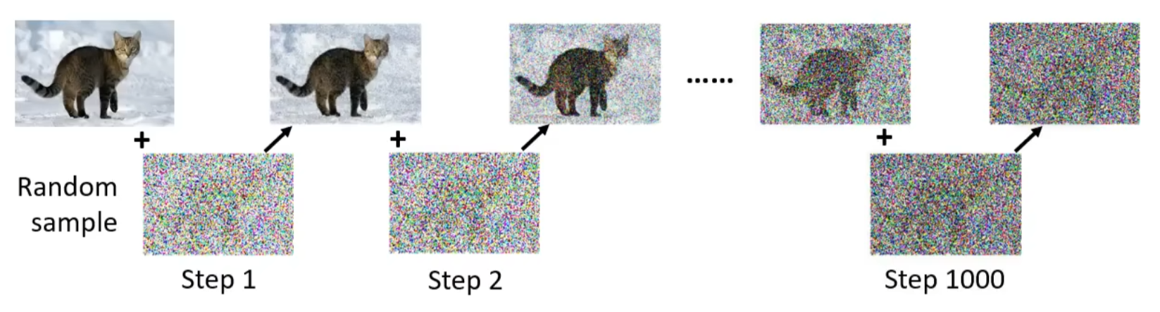
\includegraphics[width=0.8\textwidth]{figs/color/kosan.png}
    \caption{扩散过程}
    \label{fig_kuosan}
\end{figure}

在扩散过程的每一步中,图像中的噪声增加的程度是通过预定义的噪声分布实现的。每个步骤的输出即为下一个步骤的输入,逐步累积噪声直至达到预设的最大噪声水平。

上图中的每个扩散步骤都通过添加高斯噪声来实现,这些高斯噪声是通过一个简单的随机数生成器产生的。为了确保扩散过程能够准确地模拟自然图像中噪声的增加,噪声的分布和强度必须经过精确的设计和调整。

通过这种方式,扩散过程生成了大量的带噪声图像,这些图像用于训练逆扩散过程中的Denoise网络。每对训练数据中的一个部分是一个特定工作步数下的带噪声图像,另一个部分是该步数下去噪后的部分清晰图像。

在介绍了『基于扩散的图像生成模型』的基本工作流程后,我们将深入探讨该领域中最早提出的经典模型之一:DDPM。该模型由Ho等人在论文《Denoising Diffusion Probabilistic Models》\cite{hoDenoisingDiffusionProbabilistic2020a}中提出,是一种具有开创性意义的图像生成模型。DDPM\cite{hoDenoisingDiffusionProbabilistic2020a}第一个在图像生成模型中引入了『扩散过程与逆扩散过程』,奠定了基于扩散方法的图像生成技术的理论基础。通过详细推导DDPM的原理,我们可以更好地理解『基于扩散的图像生成模型』的原理。

接下来,让我们一起探讨DDPM的具体原理及其推导过程。该部分将包括三个主要内容:其一为扩散过程的原理与推导,其二为逆扩散过程的原理与推导,其三为Dnoise网络的训练。

\section{扩散过程原理与推导}

扩散过程如图\ref{fig_kuosan}所示。
扩散过程作为为Denoise网络提供训练数据的过程,在DDPM\cite{hoDenoisingDiffusionProbabilistic2020a}存在重要的作用。该部分主要将扩散过程以参数化的形式表示,通过写出该过程公式并化简的方式,从公式的角度介绍扩散过程。

\subsection{参数设定}

\begin{itemize}
    \item 原始图像:$x_0$
    \item 第 $t$ 次的从标准高斯分布中采样噪声图像: $z_t$
    \item 第$t$次将噪声$z_t$加入$x_0$后的图像:$x_t$
    \item 第$t$次加噪声时, 噪声图像$z_t$与图像$x_{t-1}$的比例$1-\alpha_t$与$\alpha_t$。$\alpha_1,\alpha_2,\cdots,\alpha_t$是一组常数,在扩散过程开始前人为设定。
\end{itemize}

\subsection{扩散过程}

\paragraph{扩散过程公式}

我们可以用符号语言描述扩散过程,如下:

1. 从数据集中获取一张原始的真实图像$x_0$

2. 从标准高斯分布$\mathcal{N}(0,1)$中采样一张噪声图$z_1$

3. 将噪声图$z_1$与原始图像$x_0$按$\sqrt{1-\alpha_1}$与$\sqrt{\alpha_1}$的比例混合, 可以得到第一步的加噪声结果, 如下所示

\begin{equation}
    x_1 = \sqrt{1-\alpha_1}z_0 + \sqrt{\alpha_1}x_0
\end{equation}

4. 将噪声图$z_2$与上一步得到的结果$z_1$按$\sqrt{1-\alpha_2}$与$\sqrt{\alpha_2}$的比例混合, 如下所示


\begin{equation}
	\begin{aligned}
		x_2 =& \sqrt{1-\alpha_2}z_1 + \sqrt{\alpha_2}x_1\\ 
	\end{aligned}
\end{equation}


5. 则第$t$张加噪图像$x_t$满足以下公式:

\begin{equation}
    x_t = \sqrt{\alpha_t}x_{t-1}+\sqrt{1-\alpha_t}z_t
\end{equation}


\paragraph{扩散过程公式简化}

\subparagraph{整体简化}

我们考察一般情况,对第$t$张加噪图像$x_t$满足的公式$x_t = \sqrt{\alpha_t}x_{t-1}+\sqrt{1-\alpha_t}z_t$进行如下变换:


\begin{equation}
\begin{aligned}
\label{fomula_f1}
x_t &= \sqrt{\alpha_t}x_{t-1}+\sqrt{1-\alpha_t}z_t\\
&= \sqrt{\alpha_t}\left(\sqrt{\alpha_{t-1}}x_{t-2}+\sqrt{1-\alpha_{t-1}}z_{t-1}\right)+\sqrt{1-\alpha_t}z_t\\
&= \sqrt{\alpha_t\alpha_{t-1}}x_{t-2}+\sqrt{\alpha_t(1-\alpha_{t-1})}z_{t-1}+\sqrt{1-\alpha_t}z_t\\
\\
&= \sqrt{\alpha_t\alpha_{t-1}}\left(\sqrt{\alpha_{t-2}}x_{t-3}+\sqrt{1-\alpha_{t-2}}z_{t-2}\right)+\sqrt{\alpha_t(1-\alpha_{t-1})}z_{t-1}+\sqrt{1-\alpha_t}z_t\\
&= \sqrt{\alpha_t\alpha_{t-1}\alpha_{t-2}}x_{t-3}+\sqrt{\alpha_t\alpha_{t-1}(1-\alpha_{t-2})}z_{t-2}+\sqrt{\alpha_t(1-\alpha_{t-1})}z_{t-1}+\sqrt{1-\alpha_t}z_t\\
\\
&=\cdots\\
&=\sqrt{\alpha_t\alpha_{t-1}\alpha_{t-2}\cdots\alpha_1}x_0+\sqrt{\alpha_t\alpha_{t-1}\cdots\alpha_2(1-\alpha_1)}z_1+\sqrt{\alpha_t\alpha_{t-1}\cdots\alpha_3(1-\alpha_2)}z_2\\
&\quad\quad\quad\quad\quad\quad\quad\quad\quad\quad+ \sqrt{\alpha_t\alpha_{t-1}\cdots\alpha_4(1-\alpha_3)}z_3+ \sqrt{\alpha_t\alpha_{t-1}\cdots\alpha_5(1-\alpha_4)}z_4\\
&\quad\quad\quad\quad\quad\quad\quad\quad\quad\quad+ \sqrt{\alpha_t\alpha_{t-1}\cdots\alpha_6(1-\alpha_5)}z_5+ \sqrt{\alpha_t\alpha_{t-1}\cdots\alpha_7(1-\alpha_6)}z_6\\
&\quad\quad\quad\quad\quad\quad\quad\quad\quad\quad\quad\quad\quad\quad\quad\vdots\\
&\quad\quad\quad\quad\quad\quad\quad\quad\quad\quad+ \sqrt{\alpha_t(1-\alpha_{t-1})}z_{t-1}+ \sqrt{1-\alpha_t}z_{t}\\
&= \underbrace{\sqrt{\alpha_t\alpha_{t-1}\alpha_{t-2}\cdots\alpha_1}x_0}_{\text{原图项}}+ \underbrace{\sum_{i=1}^t\sqrt{\alpha_t\alpha_{t-1}\cdots\alpha_{i+1}(1-\alpha_i)}z_i}_{\text{叠加噪声项}}
\end{aligned}
\end{equation}


通过上述公式\ref{fomula_f1}, 我们便可以计算经过$t$次加噪后获得的图像$x_t$. 整个公式可以看作是两个部分, 

\begin{enumerate}
    \item 其一为包含原图$x_0$的「原图项」$\sqrt{\alpha_t\alpha_{t-1}\alpha_{t-2}\cdots\alpha_1}x_0$
    \item 其二为包含$t$个噪声$z_i$的「叠加噪声项」$\sum_{i=1}^t\sqrt{\alpha_t\alpha_{t-1}\cdots\alpha_{i+1}(1-\alpha_i)}z_i$
\end{enumerate}

下面我们分别对「原图项」与「叠加噪声项」进行化简。


\subparagraph{原图项的简化}

实际上, 「原图项」是一个化简过程较为简单的项, 而后面的「叠加噪声项」是一个化简过程较为复杂的项. 现在我们探索如何简化「原图项」.

我们定义「原图项」$\sqrt{\alpha_t\alpha_{t-1}\alpha_{t-2}\cdots\alpha_1}x_0$的系数$\sqrt{\alpha_t\alpha_{t-1}\alpha_{t-2}\cdots\alpha_1}$为$\overline{\alpha_t}$,  有

\begin{equation}
    \overline{\alpha_t} = \prod\limits_{i=1}^t\alpha_i=\sqrt{\alpha_t\alpha_{t-1}\alpha_{t-2}\cdots\alpha_1} \tag{5}
\end{equation}

如$\overline{\alpha_2}=\alpha_2\cdot\alpha_1$,$\overline{\alpha_4}=\alpha_4\cdot\alpha_3\cdot\alpha_2\cdot\alpha_1$

在此定义下, 将$\overline{\alpha_t} = \prod\limits_{i=1}^t\alpha_i$代入$x_t$中的「原图项」, 有

\begin{equation}
    \begin{aligned}
        x_t &= \sqrt{\alpha_t\alpha_{t-1}\alpha_{t-2}\cdots\alpha_1}x_0+ \sum_{i=1}^t\sqrt{\alpha_t\alpha_{t-1}\cdots\alpha_{i+1}(1-\alpha_i)}z_i\\
        &= \sqrt{\overline{\alpha_t}}x_0 + \sum_{i=1}^t\sqrt{\alpha_t\alpha_{t-1}\cdots\alpha_{i+1}(1-\alpha_i)}z_i\\
    \end{aligned}
\end{equation}

\subparagraph{叠加噪声项的简化}

因为我们希望整个「叠加噪声项」是一个简单的噪声, 所以我们希望最终$x_t$满足的表达式能与其一般式$x_t = \sqrt{\alpha_t}x_{t-1}+\sqrt{1-\alpha_t}z_t$具有相同的形式。即,我们希望$x_t$的最终化简结果为$x_t=\sqrt{\overline{\alpha_t}}x_0+\sqrt{1-\overline{\alpha_t}}\widetilde{z}$的形式。 在这个形式中,叠加噪声项系数与原图项系数的平方和为$1$,与一般式保持一致;同时,我们也希望叠加噪声项的主体部分$\widetilde{z}$是一个简单的噪声,而非公式\ref{fomula_f1}中那样一堆噪声的叠加。下面正式开始对叠加噪声项的简化。

  注意到「原图项」的系数现在为$\sqrt{\overline{\alpha_t}}$, 我们期望后面的「叠加噪声项」的系数为$\sqrt{1-\overline{\alpha_i}}$, 所以对「叠加噪声项」提取系数$\sqrt{1-\overline{\alpha_t}}$, 从而有以下变化


\begin{equation}
\begin{aligned}
    \label{fomula_f2}
x_t &= \sqrt{\overline{\alpha_t}}x_0 + \sum_{i=1}^t\sqrt{\alpha_t\alpha_{t-1}\cdots\alpha_{i+1}(1-\alpha_i)}z_i\\
&= \sqrt{\overline{\alpha_t}}x_0 +\sqrt{1-\overline{\alpha_t}}\sum_{i=1}^t\frac{\sqrt{\alpha_t\alpha_{t-1}\cdots\alpha_{i+1}(1-\alpha_i)}}{\sqrt{1-\overline{\alpha_t}}}z_i
\end{aligned}
\end{equation}



现在考察上述公式\ref{fomula_f2}中的$\sum_{i=1}^t\frac{\sqrt{\alpha_t\alpha_{t-1}\cdots\alpha_{i+1}(1-\alpha_i)}}{\sqrt{1-\overline{\alpha_t}}}z_i$部分 (即上面公式中最后一个分式)以期望他是一个简单的分布。

为了方便描述,我们记这个分布为$\widetilde{z}$,即有$\widetilde{z}=\sum_{i=1}^t\frac{\sqrt{\alpha_t\alpha_{t-1}\cdots\alpha_{i+1}(1-\alpha_i)}}{\sqrt{1-\overline{\alpha_t}}}z_i$.

这个分式部分$\widetilde{z}$中的单个噪声项$z_i$均是从标准高斯分布中采样得到的, 即$z_i\sim\mathcal{N}(0,1)$(均值为0,方差为1), 且由于上一次采样的噪声不会影响下一次噪声的采样, 所以$z_i$的获取是相互独立的.

同时, 我们知道, 如果$X\sim \mathcal{N}(\mu_x,\sigma_x^2)$,$Y\sim \mathcal{N}(\mu_y,\sigma_y^2)$, 且$X$与$Y$相互独立, 则有$aX+bY\sim\mathcal{N}(a\mu_x+b\mu_y,a^2\sigma_x^2+b^2\sigma_y^2)$。

在这样的情况下, 有$\widetilde{z}$服从以下高斯分布:

\begin{equation}
    \begin{aligned}
        \widetilde{z} \sim \mathcal{N}\left[\sum_{i=1}^t\left(\frac{\sqrt{\alpha_t\alpha_{t-1}\cdots\alpha_{i+1}(1-\alpha_i)}}{\sqrt{1-\overline{\alpha_t}}}\cdot0\right), \sum_{i=1}^t\left(\frac{\alpha_t\alpha_{t-1}\cdots\alpha_{i+1}(1-\alpha_i)}{1-\overline{\alpha_t}}\cdot 1\right)\right]
    \end{aligned}
\end{equation}

可以发现, 这个高斯分布的均值部分为$0$, 因为均值部分中累加的每一项都与$0$相乘了. 从而上述高斯分布可以化简为:

\begin{equation}
    \begin{aligned}
        \widetilde{z}\sim \mathcal{N}\left(0, \sum_{i=1}^t\frac{\alpha_t\alpha_{t-1}\cdots\alpha_{i+1}(1-\alpha_i)}{1-\overline{\alpha_t}} \right)
    \end{aligned}
\end{equation}

为了搞清楚这个「叠加噪声项」到底满足什么样的高斯分布, 我们继续考察这个高斯分布的方差部分, 记为$\sigma^2_s=\sum_{i=1}^t\frac{\alpha_t\alpha_{t-1}\cdots\alpha_{i+1}(1-\alpha_i)}{1-\overline{\alpha_t}}$, 下标$s$为 sum 的缩写, 表示累加。

直接将$\sigma^2_S$拆开, 有

\begin{equation}
    \begin{aligned}
        \sigma^2_s &=\sum_{i=1}^t\frac{\alpha_t\alpha_{t-1}\cdots\alpha_{i+1}(1-\alpha_i)}{1-\overline{\alpha_t}}\\
        &=\frac{1}{1-\overline{\alpha_t}}\left[\sum_{i=1}^t\alpha_t\alpha_{t-1}\cdots\alpha_{i+1}(1-\alpha_i)\right]\\
        &\xlongequal{\text{去除累加符号}} \frac{1}{1-\overline{\alpha_t}}\left[(1-\alpha_t)+\alpha_t(1-\alpha_{t-1})+\alpha_t\alpha_{t-1}(1-\alpha_{t-2})+\cdots+\alpha_t\alpha_{t-1}\cdots\alpha_2(1-\alpha_1)\right]\\
        &\xlongequal{\text{拆除小括号}}  \frac{1}{1-\overline{\alpha_t}}\left[1-\alpha_t+\alpha_t-\alpha_t\alpha_{t-1}+\alpha_t\alpha_{t-1}-\alpha_t\alpha_{t-1}\alpha_{t-2}+\cdots+\alpha_t\alpha_{t-1}\cdots\alpha_2-\alpha_t\alpha_{t-1}\cdots\alpha_2\alpha_1\right]\\
        &=\frac{1}{1-\overline{\alpha_t}}\left[1+-\cancel{\alpha_t}+\cancel{\alpha_t}-\cancel{\alpha_t\alpha_{t-1}}+\cancel{\alpha_t\alpha_{t-1}}-\cancel{\alpha_t\alpha_{t-1}\alpha_{t-2}}+\cdots+\cancel{\alpha_t\alpha_{t-1}\cdots\alpha_2}-\alpha_t\alpha_{t-1}\cdots\alpha_2\alpha_1\right]\\
        &\xlongequal{\text{发现中括号中除了第一项和最后一项都可以消去}} \frac{1}{1-\overline{\alpha_t}}\left[1-\alpha_t\alpha_{t-1}\cdots\alpha_2\alpha_1\right]\\
        &=\frac{1}{1-\overline{\alpha_t}}(1-\overline{a_t})\\
        &\xlongequal{\text{分子分母相同}}1
    \end{aligned}
\end{equation}

也即$\sigma^2_s=1$, 从而有$\widetilde{z}=\sum_{i=1}^t\frac{\sqrt{\alpha_t\alpha_{t-1}\cdots\alpha_{i+1}(1-\alpha_i)}}{\sqrt{1-\overline{\alpha_t}}}z_i\sim\mathcal{N}(0,1)$,


至此, 我们可以发现, 「叠加噪声项」也是一个服从标准高斯分布的噪声, 从而我们可以得到第$t$步图像$x_t$与原图$x_0$之间的关系:

\begin{equation}
    \begin{aligned}
        \label{fomula_f3}
    x_t &= \sqrt{\overline{\alpha_t}}x_0 + \sum_{i=1}^t\sqrt{\alpha_t\alpha_{t-1}\cdots\alpha_{i+1}(1-\alpha_i)}z_i\\
    &= \sqrt{\overline{\alpha_t}}x_0 + \sqrt{1-\overline{a_t}}\widetilde{z},\quad \text{其中}\widetilde{z}\sim\mathcal{N}(0,1)
    \end{aligned}
\end{equation}

进行对「叠加噪声项」的化简后,我们发现实际上$t$次添加噪声的操作与直接进行一次噪声添加的效果相同。

\paragraph{扩散过程的总结}

在公式\ref{fomula_f3}的指导下, 可以立刻得到某个特定步骤$t$的加噪图像$x_t$, 且加噪图像仅与原始图像$x_0$与当前步骤数$t$有关.

经过这样的简化, 就可以简单的获取加噪后的图像, 也即训练数据了。

\paragraph{概率采样的角度看扩散过程}
\label{sec_prob}
在上面的推导中, 我们得出了直接从原图$x_0$获取第$t$次后的加噪图像$x_t$的公式如下:

\begin{equation}
    \begin{aligned}
        \label{fomula_f4}
        x_t= \sqrt{\overline{\alpha_t}}x_0 + \sqrt{1-\overline{a_t}}\widetilde{z},\quad \text{其中}\widetilde{z}\sim\mathcal{N}(0,1)
    \end{aligned}
\end{equation}

实际上, 我们也可以将$x_t$看作是某种概率的采样结果, 推导如下:

已知$\widetilde{z}\sim\mathcal{N}(0,1)$, 则有$\sqrt{1-\overline{a_t}}\widetilde{z}\sim\mathcal{N}(0,1-\overline{\alpha_t})$

从而有$\sqrt{\overline{\alpha_t}}x_0 + \sqrt{1-\overline{a_t}}\widetilde{z}\sim\mathcal{N}(\sqrt{\overline{\alpha_t}}x_0,1-\overline{\alpha_t})$ , 

从而有$q(x_t\vert x_0)\sim \mathcal{N}(\sqrt{\overline{\alpha_t}}x_0,1-\overline{\alpha_t})$

这个结果表明,第$t$步的加噪图像$x_t$​可以看作是从一个正态分布中采样的结果,其均值和方差分别由初始图像$x_0$和累积噪声参数$\overline{\alpha_t}$​决定

同理, 由于有$x_t = \sqrt{\alpha_t}x_{t-1}+\sqrt{1-\alpha_t}z_t$, 所以有 

\begin{equation}
    \begin{aligned}
        q(x_t|x_{t-1},x_0)\sim \mathcal{N}(\sqrt{\alpha_t}x_{t-1}, 1-\alpha_t)
    \end{aligned}
\end{equation}


从概率的角度理解扩散过程有助于下面对于逆扩散过程的推导。
\section{逆扩散过程原理与推导}

很显然, 我们想要通过$x_t$来预测$x_{t-1}$. 

如果我们能够逆转上述扩散过程, 并从$p(x_{t-1}|x_t)$采样,就可以从高斯噪声$x_t\sim N(0,1)$还原出原图服从的分布$x_0\sim p(x)$。

如何获得$p_\theta(x_{t-1}\vert x_t)$这个概率密度 (式子中的$\theta$表示神经网络的参数)就是一个需要探讨的问题. 直接计算比较困难, 所以我们可以考虑对公式进行变形. 对公式使用贝叶斯公式, 有如下结果


\begin{equation}
\begin{aligned}
p_\theta(x_{t-1}|x_t) &\xlongequal{\text{贝叶斯公式}} \frac{p_\theta(x_{t-1},x_t)}{p(x_t)}\\
&\xlongequal{\text{分母用全概率公式展开}} \frac{p(x_t|x_{t-1})\cdot p_\theta(x_{t-1})}{p(x_t)}\\
&=p(x_t|x_{t-1}) \cdot \frac{p_\theta(x_{t-1})}{p(x_t)}\\
\end{aligned}
\end{equation}


通过这样的变换, 我们将一个无法计算的式子$p_\theta(x_{t-1}|x_t)$, 改写成了一个可计算的部分$p(x_t|x_{t-1})$和一个不可计算的分式$\frac{p_\theta(x_{t-1})}{p(x_t)}$的乘积

自己观察这个不可计算的分式, 可以发现, 这个分式的分子与分母都是不可计算的. 因为如果我们能直接得到$p(x_{t})$或$p(x_{x-1})$, 那我们就能直接得出$p(x_0)$. 但是我们计算$p (x_{t-1}|x_t)$的目的就是为了计算$p(x_0)$, 如果可以直接得出$p(x_0)$, 那么我们就没有计算$p (x_{t-1}|x_t)$, 所以我们不可能直接得到$p(x_t)$.

可以想到, 虽然直接计算$p(x_t)$是不可行的, 但是计算$p(x_t|x_0)$是十分简单的, 在\ref{sec_prob} 中我们介绍过这个计算:

$$
p(x_t\vert x_0)\sim \mathcal{N}(\sqrt{\overline{\alpha_t}}x_0,1-\overline{\alpha_t})
$$

所以我们可以考虑将$p(x_t)$的计算转换成$p(x_t|x_0)$用于计算, 由此可以计算$p_\theta(x_{t-1}|x_t,x_0)$, 有



\begin{equation}
\begin{aligned}
p_\theta(x_{t-1}|x_t,x_0) &\xlongequal{\text{贝叶斯公式}} \frac{p_\theta(x_{t-1},x_t,x_0)}{p(x_t,x_0)}\\
&\xlongequal{\text{分子用全概率公式展开}} \frac{p(x_t|x_{t-1},x_0)\cdot p_\theta(x_{t-1},x_0)}{p(x_t,x_0)}\\
&=p(x_t|x_{t-1}) \cdot \frac{p(x_{t-1},x_0)}{p(x_t,x_0)}\\
&=p(x_t|x_{t-1}) \cdot \frac{p(x_{t-1},x_0)}{p(x_t,x_0)}\\
=& p(x_t|x_{t-1}) \cdot \frac{p(x_{t-1}|x_0)\cdot p(x_0)}{p(x_t|x_0)\cdot p(x_0)}\\
=& p(x_t|x_{t-1}) \cdot \frac{p(x_{t-1}|x_0)}{p(x_t|x_0)}\\
\end{aligned}
\end{equation}


对上述推导取等式左侧与右侧第一项, 有 $p_\theta(x_{t-1}|x_t,x_0)=p(x_t|x_{t-1}) \cdot \frac{p_\theta(x_{t-1}|x_0)}{p(x_t|x_0)}$

可能有人发现, 在第三个等式中, 我们直接将 $p(x_t|x_{t-1},x_0)$ 替换为了 $p(x_t|x_{x-1})$, 这可以用马尔可夫性(Markov property)来解释:马尔可夫性假设指出,一个状态只依赖于前一个状态,而与更早的状态条件独立。应用于 DDPM 模型,这意味着:

$p(x_t|x_{t-1},x_0)=p(x_t|x_{t-1})p(x_t | x_{t-1}, x_0) = p(x_t | x_{t-1})p(x_t|x_{t-1},x_0)=p(x_t|x_{t-1})$

这三项就都是很好计算的项了, 虽然此处我们使用的是$p(x_{t}|x_{t-1})$而非$q(x_t|x_{t-1})$, 但他们之间表示的内容是一致的, 均表示前向过程中的加噪.

从\ref{sec_prob}中, 我们有推导结果


\begin{equation}
    \begin{aligned}
        p(x_t|x_{t-1},x_0)= q(x_t|x_{t-1},x_0)&\sim \mathcal{N}(\sqrt{\alpha_t}x_{t-1}, 1-\alpha_t)\\
        &=\frac{1}{\sqrt{2\pi}\sigma}e^{-\frac{1}{2}\cdot(\frac{x_t-\mu}{\sigma})^2}\\
        &= \frac{1}{\sqrt{2\pi}\cdot\sqrt{1-\alpha_t}}\exp\left[{-\frac{1}{2}\cdot\left(\frac{x_t-\sqrt{\alpha_t}x_{t-1}}{\sqrt{1-\alpha_t}}\right)^2}\right]\\
        \text{$x_t$为随机变量}
    \end{aligned}
\end{equation}

\begin{equation}
    \begin{aligned}
        p_\theta(x_{t-1}\vert x_0)=q(x_{t-1}\vert x_0)&\sim \mathcal{N}(\sqrt{\overline{\alpha_t}}x_0,1-\overline{\alpha_{t-1}})\\
        &=\frac{1}{\sqrt{2\pi}\sigma}e^{-\frac{1}{2}\cdot(\frac{x_{t-1}-\mu}{\sigma})^2}\\
        &= \frac{1}{\sqrt{2\pi}\cdot\sqrt{1-\overline{\alpha_{t-1}}}}\exp\left[{-\frac{1}{2}\cdot\left(\frac{x_{t-1}-\sqrt{\overline{\alpha_{t-1}}}x_0}{\sqrt{1-\overline{\alpha_{t-1}}}}\right)^2}\right]\\
        &\text{$x_{t-1}$为随机变量}
    \end{aligned}
\end{equation}


\begin{equation}
    \begin{aligned}
        p(x_t\vert x_0)=q(x_t\vert x_0)&\sim \mathcal{N}(\sqrt{\overline{\alpha_t}}x_0,1-\overline{\alpha_t})\\
        &=\frac{1}{\sqrt{2\pi}\sigma}e^{-\frac{1}{2}\cdot(\frac{x_t-\mu}{\sigma})^2}\\
        &= \frac{1}{\sqrt{2\pi}\cdot\sqrt{1-\overline{\alpha_t}}}\exp\left[{-\frac{1}{2}\cdot\left(\frac{x_t-\sqrt{\overline{\alpha_t}}x_0}{\sqrt{1-\overline{\alpha_t}}}\right)^2}\right]\\
        &\text{$x_t$为随机变量}
    \end{aligned}
\end{equation}


将这三个式子带入上述公式$p_\theta(x_{t-1}|x_t,x_0)=p(x_t|x_{t-1}) \cdot \frac{p_\theta(x_{t-1}|x_0)}{p(x_t|x_0)}$, 有如下化简:


\begin{equation}
    \begin{aligned}
        p_\theta(x_{t-1}|x_t,x_0) &= p(x_t|x_{t-1}) \cdot \frac{p_\theta(x_{t-1}|x_0)}{p(x_t|x_0)}\\
        &= \frac{1}{\sqrt{2\pi}\cdot\sqrt{1-\alpha_t}}\exp\left[{-\frac{1}{2}\cdot\left(\frac{x_t-\sqrt{\alpha_t}x_{t-1}}{\sqrt{1-\alpha_t}}\right)^2}\right]\cdot\frac{\frac{1}{\sqrt{2\pi}\cdot\sqrt{1-\overline{\alpha_{t-1}}}}\exp\left[{-\frac{1}{2}\cdot\left(\frac{x_{t-1}-\sqrt{\overline{\alpha_{t-1}}}x_0}{\sqrt{1-\overline{\alpha_{t-1}}}}\right)^2}\right]}{\frac{1}{\sqrt{2\pi}\cdot\sqrt{1-\overline{\alpha_t}}}\exp\left[{-\frac{1}{2}\cdot\left(\frac{x_t-\sqrt{\overline{\alpha_t}}x_0}{\sqrt{1-\overline{\alpha_t}}}\right)^2}\right]}\\
        &\xlongequal[\text{忽略前面的系数}]{\text{指数相乘(除)等于幂相加(减)}}k\cdot\exp\left\{-\frac12\cdot\left[ \left(\frac{x_t-\sqrt{\alpha_t}x_{t-1}}{\sqrt{1-\alpha_t}}\right)^2 +\left(\frac{x_{t-1}-\sqrt{\overline{\alpha_{t-1}}}x_0}{\sqrt{1-\overline{\alpha_{t-1}}}}\right)^2- \left(\frac{x_t-\sqrt{\overline{\alpha_t}}x_0}{\sqrt{1-\overline{\alpha_t}}}\right)^2 \right]\right\}\\
    \end{aligned}
\end{equation}


这个公式看起来很复杂, 但是我们可以这样考虑:整个公式为一个常数与一个「以$e$为底的指数」的乘积, 与高斯分布的形式很像, 而我们知道, 高斯分布中的指数部分是一个完全平方:$\exp\left(-\frac12\cdot\left[\frac{(x-\mu)}{\sigma}\right]^2\right)=\exp\left\{-\frac12\left(\frac{1}{\sigma^2}x^2-\frac{2\mu}{\sigma^2}x+\frac{\mu^2}{\sigma^2}\right)\right\}$, 所以我们可以也将上面公式中的指数部分变成一个完全平方. 

根据上面的思想,我们可以有如下推导:

\begin{equation}
    \begin{aligned}
        p_\theta(x_{t-1}|x_t,x_0) &= k\cdot \exp{\left\{-\frac{1}{2}\cdot\left[\left(\frac{x-\sqrt{\alpha_t}x_{t-1}}{\sqrt{1-\alpha_t}}\right)^2+\left(\frac{x-\sqrt{\overline{\alpha_{t-1}}}x_0}{\sqrt{1-\overline{\alpha_{t-1}}}}\right)^2-\left(\frac{x-\sqrt{\overline{\alpha_t}}x_0}{\sqrt{1-\overline{\alpha_t}}}\right)^2   \right]\right\}}\\
        &\Downarrow\text{将等式右侧平方拆开}\\
        \text{原式} &=k\cdot\exp \left\{ -\frac{1}{2}\left(\frac{{x}_{t}^{2}-2 \sqrt{\alpha_{t}} {x}_{t} {x}_{t-1}+\alpha_{t} {x}_{t-1}^{2}}{1-\alpha_{t}}+\frac{{x}_{t-1}^{2}-2 \sqrt{\overline{\alpha_{t-1}}} {x}_{0} {x}_{t-1}+\overline{\alpha_{t-1}} {x}_{0}^{2}}{1-\overline{\alpha_{t-1}}}-\frac{\left({x}_{t}-\sqrt{\overline{\alpha_{t}}} {x}_{0}\right)^{2}}{1-\overline{\alpha_{t}}}\right)\right\} \\
        &\Downarrow\text{合并等式右侧$x_{t-1}$的同类项}\\
        \text{原式} &=k\cdot\exp \left\{\underbrace{-\frac{1}{2}\left[\left(\frac{\alpha_{t}}{1-\alpha_{t}}+\frac{1}{1-\overline{\alpha_{t-1}}}\right) {x}_{t-1}^{2}-2\left(\frac{ \sqrt{\alpha_{t}}}{1-\alpha_{t}} {x}_{t}+\frac{\sqrt{\overline{\alpha_{t-1}}}}{1-\overline{\alpha_{t-1}}} {x}_{0}\right) {x}_{t-1}+C\left({x}_{t}, {x}_{0}\right)\right]}_{\text{这部分就是高斯分布中的}-\frac12\left(\frac{1}{\sigma^2}x^2-\frac{2\mu}{\sigma^2}x+\frac{\mu^2}{\sigma^2}\right)} \right\}\\
        &\xlongequal{\text{完全平方公式}}k\cdot\exp\left\{-\frac{1}{2}\cdot\left[  \frac{x_{t-1}-\left(\frac{\sqrt{\alpha_t}(1-\overline{\alpha_{t-1}})}{1-\overline{\alpha_t}}x_t+\frac{\sqrt{\overline{\alpha_{t-1}}}\left(1-\alpha_t\right)}{1-\overline{\alpha_t}}x_0\right)}{\sqrt{\frac{\alpha_t}{1-\alpha_t}+\frac{1}{1-\overline{\alpha_{t-1}}}}}  \right]^2\right\}\\
        &=\exp\left(-\frac12\cdot\left[\frac{(x-\mu)}{\sigma}\right]^2\right)\\
    \end{aligned}
\end{equation}


其中,$\mu=\frac{\sqrt{\alpha_t}(1-\overline{\alpha_{t-1}})}{1-\overline{\alpha_t}}x_t+\frac{\sqrt{\overline{\alpha_{t-1}}}\left(1-\alpha_t\right)}{1-\overline{\alpha_t}}x_0$,$\sigma=\sqrt{\frac{\alpha_t}{1-\alpha_t}+\frac{1}{1-\overline{\alpha_{t-1}}}}$

通过以上化简, 我们轻易的得到的$p_\theta(x_{t-1}|x_t,x_0)$所服从的分布实际上也是一个高斯分布, 即

$$p_\theta(x_{t-1}|x_t,x_0)\sim\mathcal{N}(\mu,\sigma^2)\sim\mathcal{N}\left(\frac{\sqrt{\alpha_t}(1-\overline{\alpha_{t-1}})}{1-\overline{\alpha_t}}x_t+\frac{\sqrt{\overline{\alpha_{t-1}}}\left(1-\alpha_t\right)}{1-\overline{\alpha_t}}x_0, \frac{\alpha_t}{1-\alpha_t}+\frac{1}{1-\overline{\alpha_{t-1}}}\right)$$

观察方差$\sigma^2=\frac{\alpha_t}{1-\alpha_t}+\frac{1}{1-\overline{\alpha_{t-1}}}$可以发现, 其中所有的值均为常数, 是一个可以直接计算的值

观察均值$\mu=\frac{\sqrt{\alpha_t}(1-\overline{\alpha_{t-1}})}{1-\overline{\alpha_t}}x_t+\frac{\sqrt{\overline{\alpha_{t-1}}}\left(1-\alpha_t\right)}{1-\overline{\alpha_t}}x_0$, 可以发现所有的$\alpha$均是已知值,$x_t$也是已知值, 而整个均值的式子中, 唯一一个不知道的值为$x_0$. 如果能得知$x_0$就能很快的进行计算了.

实际上, 我们在\ref{sec_prob}中有扩散过程的公式\ref{fomula_f4}如下

$$x_t=\sqrt{\overline{\alpha_t}}x_0 + \sqrt{1-\overline{a_t}}\widetilde{z},\quad \text{其中}\widetilde{z}\sim\mathcal{N}(0,1)$$

从这个式子中, 我们可以通过移项的方式,反推出$x_0$,即$x_0 = \frac{1}{\sqrt{\overline{\alpha_t}}}\left(x_{t-1}-\sqrt{1-\overline{\alpha_t}}\widetilde{z}\right)$,用这个值替换$\mu$中的$x_0$, 有如下结果:


\begin{equation}
\begin{aligned}
\mu&=\frac{\sqrt{\alpha_t}(1-\overline{\alpha_{t-1}})}{1-\overline{\alpha_t}}x_t+\frac{\sqrt{\overline{\alpha_{t-1}}}\left(1-\alpha_t\right)}{1-\overline{\alpha_t}}x_0\\
&=\frac{\sqrt{\alpha_t}(1-\overline{\alpha_{t-1}})}{1-\overline{\alpha_t}}x_t+\frac{\sqrt{\overline{\alpha_{t-1}}}\left(1-\alpha_t\right)}{1-\overline{\alpha_t}}\cdot\frac{1}{\sqrt{\overline{\alpha_t}}}\left(x_{t-1}-\sqrt{1-\overline{\alpha_t}}\widetilde{z}\right)\\
&=\frac{1}{\sqrt{\alpha_t}}\left( x_t-\frac{1-\alpha_t}{\sqrt{1-\overline{\alpha_t}}}\widetilde{z} \right)
\end{aligned}
\end{equation}


即

$$
\mu=\frac{1}{\sqrt{\alpha_t}}\left( x_t-\frac{1-\alpha_t}{\sqrt{1-\overline{\alpha_t}}}\widetilde{z} \right)
$$

整个式子中仅有$\widetilde{z}$是一个不可直接获得的值了. 为何会出现一个不能直接获得的$\widetilde{z}$呢?回顾上述过程发现, 这个$\widetilde{z}$是在为了消去$x_0$时引入的一个值. 这个$\widetilde{z}$表示的是在获得$x_t$的过程中,  向$x_0$中加入的噪声. 

为了能够获得这个噪声, 原文使用了一个神经网络进行预测.

在使用神经网络获得$\widetilde{z}$后,$\mu$与$\sigma^2$都变的可以计算, 从而$p_\theta(x_{t-1}|x_t,x_0)\sim \mathcal{N}(\mu, \sigma^2)$就变成了可以直接获得的高斯分布. 从而$x_{t-1}$就可以轻松的从这个分布中采样获取了.
这个神经网络就是\ref{sec_inverse}逆扩散过程中所说的Denoise网络,也即我们下面将要介绍的噪声预测器。

\section{噪声预测器的训练}

在 DDPM 中, 使用 UNet 网络进行噪声图像的预测, 并采样极大似然函数作为损失函数进行预测。

首先我们介绍一下极大似然函数与极大似然估计。

\subsection{极大似然函数与极大似然估计}

实际上,这一部分对于没有思考过极大似然估计背后原理的读者可能有些难懂,所以本人推荐观看bilibili网站中视频博主“小崔说数”关于极大似然估计的讲解\cite{XiaoCuiShuoShuShiFenZhongGaoDingZuiDaSiRanGuJi2021},此处简单记录关于视频内容的理解。

极大似然估计(Maximum Likelihood Estimation,MLE)是统计学中用于估计模型参数的一种方法,这个方法适用于已经得知样本所服从的分布时,估计这个分布中参数的情况。它基于这样一个简单而强有力的想法:小概率事件在现实中几乎不发生。因此,当我们观测到某种事件发生时,这个事件在其所服从的分布中应该是一个大概率事件。

具体来说,假设我们有一个概率分布模型,它依赖于一些未知参数,我们的任务是根据观测数据来估计这些参数。假设我们观测到了 \(n\) 个独立同分布的数据点 \(x_1, x_2, \ldots, x_n\),并且我们知道数据服从一个参数为 \(\theta\) 的概率分布 \(P(x|\theta)\)。

极大似然估计的核心思想是选择使得观测数据出现的概率最大的参数 \(\theta\)。这意味着我们需要找到一个参数 \(\theta\) 使得所有观测到的事件的联合概率最大化。

1. 似然函数:首先,我们定义似然函数(Likelihood Function),它表示在参数 \(\theta\) 下,观测数据 \(x_1, x_2, \ldots, x_n\) 出现的联合概率。对于独立同分布的数据,似然函数可以表示为:
   \[
   L(\theta) = P(x_1, x_2, \ldots, x_n | \theta) = \prod_{i=1}^n P(x_i | \theta)
   \]

2. 最大化似然函数:我们的目标是找到参数 \(\theta\) 使得似然函数 \(L(\theta)\) 最大。由于乘积运算复杂,我们通常对似然函数取对数,将其转化为对数似然函数(Log-Likelihood Function):
   \[
   \ell(\theta) = \log L(\theta) = \log \left( \prod_{i=1}^n P(x_i | \theta) \right) = \sum_{i=1}^n \log P(x_i | \theta)
   \]
   取对数不会改变最大值的位置,但使得计算更为简便。

3. 求解最优参数:我们通过求解对数似然函数 \(\ell(\theta)\) 的最大值来找到最优参数 \(\theta\)。这通常涉及对 \(\theta\) 求导,并找到导数为零的点,即:
   \[
   \frac{\partial \ell(\theta)}{\partial \theta} = 0
   \]
   导数为$0$的点为函数的极值点,当$\theta$为极值点时,对应的$\ell(\theta)$便可能达到最大值,及联合概率密度达到最大值。这说明,当$\theta$为极值点,从这个概率分布中取得样本为我们所观测数据的概率达到最大值

极大似然估计方法可以解释为:在所有可能的参数值中,我们选择这样一个参数,使得实际观测到的数据在该参数下的出现概率最大。换句话说,这个参数使得观测到的数据最符合模型的假设。因此,极大似然估计本质上是在寻找最能解释观测数据的参数。

总之,极大似然估计是一种通过最大化观测数据在模型下出现的概率来估计参数的方法。它基于一个直观的想法,即观测到的事件应该是高概率事件,因此选择使观测数据出现概率最大的参数,就是最符合数据的参数。

\subsection{利用极大似然函数进行参数迭代}

我们知道, 极大似然估计在参数估计时, 使用的是这样的想法:小概率事件在现实中几乎不发生. 所以如果我们观测到某种事件发生了, 则说明这个事件所服从的分布中, 已经发生的这个事件一定是一个大概率事件. 能将所有已发生的事件的概率都最大化的参数, 也就是使似然函数最大的参数, 则是我们需要的参数.

从另一个角度说, 如果似然函数 $L$ 越大, 则说明当前取得的参数越合理.  

所以我们使用似然函数 $L$ 作为似然函数, 将最大化似然函数 $\max L$ 作为训练的目标. 

\subsubsection{复习极大似然函数的构建过程}

我们先用一个简单例子复习一下极大似然函数的构建过程. 如果你对极大似然估计很熟悉的话, 可以跳过这一部分. 

如果下一部分中构建似然函数的过程难以理解, 可以与这一个简单的例子进行类比.

\begin{enumerate}
    \item 现在有这样一个场景\begin{enumerate}
        \item 我们有一个装了不知道多少个黑白小球的袋子 (是一个满足二项分布的模型)
        \begin{enumerate}
            \item 取得黑球的概率为 $\theta$, 取得白球的概率为 $1-\theta$ 
        \end{enumerate}
        \item 现在进行 $5$ 次采样, 有结果如下:
        \begin{enumerate}
            \item  采样 1:黑
            \item  采样 2:黑
            \item  采样 3:黑
            \item  采样 4:白
            \item  采样 5:白
        \end{enumerate}
        \item 问这个二项分布的参数 $\theta$ 是多少
    \end{enumerate}
    \item 采样与二项分布
    \begin{enumerate}
        \item 对于采样 1, 摸到了黑球, 在二项分布中有概率为 $\theta$ 
        \item 对于采样 2, 摸到了黑球, 在二项分布中有概率为 $\theta$ 
        \item 对于采样 3, 摸到了黑球, 在二项分布中有概率为 $\theta$ 
        \item 对于采样 4, 摸到了白球, 在二项分布中有概率为 $1-\theta$ 
        \item 对于采样 5, 摸到了白球, 在二项分布中有概率为 $1-\theta$ 
        \item 对于整个五次采样结果为 (黑、黑、黑、白、白) 的概率为:$\theta^3\cdot(1-\theta)^2$ 
    \end{enumerate}
    \item 极大似然估计的思想
    \begin{enumerate}
        \item 既然五次采样出现了这样的结果, 所以我们认为发生这种 (黑、黑、黑、白、白) 情况的概率应该是最大的 (因为小概率事件不可能发生)
    \end{enumerate}
    \item 极大似然估计
    \begin{enumerate}
        \item 所以我们认为, $\theta$ 一定能使采样概率 $\theta^3\cdot(1-\theta)^2$ 取到最大值.
        \item 也即, 一个能使概率 $\theta^3\cdot(1-\theta)^2$ 达到最大值的 $\theta$ 是一个合理的 $\theta$
        \item 所以应该求 $\theta^3\cdot(1-\theta)^2$ 取最大值时, $\theta$ 的取值.
        \item 因为 $\theta^3\cdot(1-\theta)^2$ 是一个高次幂的式子, 难以计算, 我们我们转而计算 $L(\theta)=\log\left[ \theta^3\cdot (1-\theta)^2 \right]$ 
        \item $L(\theta)=\log\left[ \theta^3\cdot (1-\theta)^2 \right]$ 即为似然函数
    \end{enumerate}
\end{enumerate}

\subsubsection{扩散模型场景与极大似然估计}

当我们复习了一个简单情形的似然估计的用法后, 可以快速的类比到当前的扩散模型任务中.

\begin{enumerate}
    \item 现在我们有扩散模型的场景
    \begin{enumerate}
        \item 我们有一个装了不知道多少个各异图像的图像集 (是一个满足 $p_\theta(x_{t-1}|x_t)$ 的模型)
        \begin{enumerate}
            \item 取得图像 $x_t$ 的概率为 $p_\theta(x_{t-1}|x_t)$ , $t=1,2,3,\cdots,T-1$
            \item 取得图形 $x_T$ 的概率为 $p(x_T)\sim\mathcal{N}(0,1)$
        \end{enumerate}
        \item 现在进行 $T$ 次采样, 有结果如下
        \begin{enumerate}
            \item 采样 0:$x_0$ 
            \item 采样 1:$x_1$ 
            \item 采样 2:$x_3$ 
            \item $\cdots$ 
            \item 采样 $t$:$x_t$ 
            \item $\cdots$
            \item 采样 $T$:$x_T$ 
        \end{enumerate}
        \item 问这个概率模型 $p_\theta(x_{t}|x_{t+1})$ 中的 $\theta$ 是多少
    \end{enumerate}
    \item 采样与二项分布
    \begin{enumerate}
        \item 对于采样 0, 获得了图像 $x_0$, 在分布中有概率 $p_\theta(x_0|x_1)$
        \item 对于采样 1, 获得了图像 $x_1$, 在分布中有概率 $p_\theta(x_1|x_2)$.
        \item $\cdots$
        \item 对于采样 t, 获得了图像 $x_{t}$, 在分布中有概率 $p_\theta(x_{t}|x_{t+1})$.
        \item $\cdots$
        \item 对于采样 $T-1$, 获得了图像 $x_{T-1}$, 在分布中有概率 $p_\theta(x_{T-1}|x_T)$ 
        \item 对于采样 $T$, 获得了图像 $x_{T}$, 在分布中有概率 $p(x_T)\sim\mathcal N (0,1)$. 
        \item 因为 $x_T$ 是直接从标准高斯分布中获取的, 所以下标中没有 $\theta$ 
        \item 对于整个 $T$ 次采样结果为 $(x_0,x_1,x_2,\cdots,x_T)$ 的概率为
        
        $$p (x_T)\cdot p_\theta(x_{T-1}|x_T)\cdot p_\theta(x_{T-2}|x_{T-1})\cdots p_\theta(x_1|x_2)\cdot p (x_0|x_1)$$
    \end{enumerate}
    \item 极大似然估计的思想
    \begin{enumerate}
        \item 既然 $T$ 次采样出现了这样的结果, 所以我们认为发生这种 $(x_0,x_1,x_2,\cdots,x_T)$ 情况的概率应该是最大的 (因为小概率事件不可能发生)
    \end{enumerate}
    \item 极大似然估计
    \begin{enumerate}
        \item 所以我们认为, $\theta$ 一定能使采样概率 $p (x_T)\cdot p_\theta(x_{T-1}|x_T)\cdot p_\theta(x_{T-2}|x_{T-1})\cdots p_\theta(x_1|x_2)\cdot p_\theta(x_0|x_1)$ 取到最大值.
        \item 也即, 一个能使上述概率达到最大值的 $\theta$ 是一个合理的 $\theta$
        \item 所以应该求 $p (x_T)\cdot p_\theta(x_{T-1}|x_T)\cdot p_\theta(x_{T-2}|x_{T-1})\cdots p_\theta(x_1|x_2)\cdot p_\theta(x_0|x_1)$ 取最大值时, $\theta$ 的取值.
        \item 因为 $p (x_T)\cdot p_\theta(x_{T-1}|x_T)\cdot p_\theta(x_{T-2}|x_{T-1})\cdots p_\theta(x_1|x_2)\cdot p_\theta (x_0|x_1)$ 是一个高次幂的式子, 难以计算, 我们我们转而计算 $L(\theta)=\log\left[ p (x_T)\cdot p_\theta(x_{T-1}|x_T)\cdot p_\theta(x_{T-2}|x_{T-1})\cdots p_\theta(x_1|x_2)\cdot p_\theta (x_0|x_1) \right]$ 
        \item $L(\theta)=\log\left[ p (x_T)\cdot p_\theta(x_{T-1}|x_T)\cdot p_\theta(x_{T-2}|x_{T-1})\cdots p_\theta(x_1|x_2)\cdot p_\theta (x_0|x_1) \right]$ 即为似然函数
    \end{enumerate}
\end{enumerate}

实际上, 我们不可能简单的仅仅采样一个 $x_0$, 数据集中的所有图像都应该是一个可能的 $x_0$

所以我们要对式子 $p (x_T)\cdot p_\theta(x_{T-1}|x_T)\cdot p_\theta(x_{T-2}|x_{T-1})\cdots p_\theta(x_1|x_2)\cdot p (x_0|x_1)$ 进行积分, 有如下结果

\begin{equation}
\begin{aligned}
    P_\theta(x_0)=\int\limits_{x_1:x_T}p (x_T)\cdot p_\theta(x_{T-1}|x_T)\cdot p_\theta(x_{T-2}|x_{T-1})\cdots p_\theta(x_1|x_2)\cdot p_\theta (x_0|x_1)dx_1:x_T
\end{aligned}
\end{equation}

所以有对数似然函数

\begin{equation}
\begin{aligned}
    L(\theta)=\log P_\theta(x_0)=\log\left(\int\limits_{x_1:x_T}p (x_T)\cdot p_\theta(x_{T-1}|x_T)\cdot p_\theta(x_{T-2}|x_{T-1})\cdots p_\theta(x_1|x_2)\cdot p_\theta (x_0|x_1)dx_1:x_T\right)
\end{aligned}
\end{equation}

但实际上, 这个似然函数的计算比较困难, 所以在训练时不会直接进行计算.

那么该如何计算这个似然函数呢?请看下面的部分.

\subsubsection{最大化似然函数的下界}

由于 DDPM 的过程有些复杂, 一共经过了 $t$ 次的去噪, 比较复杂. 所以我们构建一个只有一个加噪过程的 DDPM 模型用来推导 (实际上这个「只有一个加噪过程的 DDPM」就是变分自编码器 VAE)

\paragraph{单个Denoise过程的DDPM}

由于只有一个加噪过程, 所以有似然函数如下:

\begin{equation}
\begin{aligned}
    \log P_\theta(x)=\log\int\limits_{x_1}p(x_1)p_{\theta}(x_0|x_1)dx_1
\end{aligned}
\end{equation}



从而可以有以下推导:


\begin{equation}
\begin{aligned}
\log P_\theta(x)&=\log\int\limits_{x_1}p(x_1)p_{\theta}(x_0|x_1)dx_1\\
&=\log\int\limits_{x_1}p_\theta(x_0,{x_1})d{x_1}\\
&=\log\int\limits_{x_1}\frac{q(x_1|x_0)}{q({x_1}|x_0)}p_\theta(x_0,{x_1})d{x_1}\\
&=\log\int\limits_{x_1}q(x_1|x_0)\frac{p_\theta(x_0,x_1)}{q(x_1|x_0)}dx_1\\
&=\log \mathbb{E}_{q(x_1|x_0)}\left[\frac{p_\theta(x_0,x_1)}{q(x_1|x_0)}\right]\\
&\ge \mathbb{E}_{q(x_1|x_0)}\left[\log\frac{p_\theta(x_0,x_1)}{q(x_1|x_0)}\right]\quad\quad[\text{琴生不等式, 如果函数}\varphi\text{为凹函数, 则有}\varphi\left(\mathbb{E}(x)\right)\ge\mathbb{E}\left(\varphi(x)\right)]
\end{aligned}
\end{equation}


我们将 $p_\theta(x_0,x_1)$ 替换为 $p_\theta(x_0|x_1)p(x_1)$ , 则有


\begin{equation}
\begin{aligned}
\mathbb{E}_{q(x_1|x_0)}\left[\log\frac{p_\theta(x_0,x_1)}{q(x_1|x_0)}\right]&=\mathbb{E}_{q(x_1|x_0)}\left[\log\frac{p_\theta(x_0|x_1)p(x_1)}{q(x_1|x_0)}\right]\\
&=\mathbb{E}_{q(x_1|x_0)}\left[\log{ p_\theta(x_0|x_1) }+\log{p(x_1)}-\log{q(x_1|x_0)}\right]\\
&=\mathbb{E}_{q(x_1|x_0)}\left[\log{ p_\theta(x_0|x_1) }\right]-\text{KL}\left[q(x_1|x_0)\Vert p(x_1)\right]\\
\end{aligned}
\end{equation}


这个式子分为了两项, 其中
\begin{enumerate}
    \item 第一项 $\mathbb{E}_{q(x_1|x_0)}\left[\log{ p_\theta(x_0|x_1) }\right]$ 是一个期望值,它表示的是给定潜在变量 $x_1$ 后生成原始图像 $x_0$ 的对数似然。这个期望, 也即其下标 $q(x_1|x_0)$ 表示前向过程, 是一个已知的过程 , 所以我们可以通过采样 $x_1$ 来近似计算这个期望值
    \item 第二项 $\text{KL}\left[q(x_1|x_0)\Vert p(x_1)\right]$ 是是两个已知分布之间的 KL 散度。而经过上面的计算, 我们知道 $q(x_1|x_0)$ 与 $p(x_1)$ 均服从正态分布, 这使得 KL 散度可以解析计算 (两个正态分布之间的 KL 散度可以用公式直接计算).
\end{enumerate}

从而整个变分下界可以计算. 通过最大化这个变分下界的形式, 我们可以最大化似然函数, 找到最适合的 $\theta$ 值.


\paragraph{多个Denoise过程的DDPM}

我们只需要将「单个Denoise过程的DDPM」中的 $x_1$ 变成 $x_0:x_T$ 即可得到 DDPM 的推导过程.

根据上面的推导, 我们知道 DDPM 有似然函数如下:

\begin{equation}
\begin{aligned}
	\log P_\theta(x_0)=\log\left[\int\limits_{x_1:x_T}p (x_T)\cdot p_\theta(x_{T-1}|x_T)\cdot p_\theta(x_{T-2}|x_{T-1})\cdots p_\theta(x_1|x_2)\cdot p_\theta (x_0|x_1)dx_1:x_T\right]
\end{aligned}
\end{equation}


从而有以下推导:

\begin{equation}
    \begin{aligned}
	\log P_\theta(x_0)&=\log\left[\int\limits_{x_1:x_T}p (x_T)\cdot p_\theta(x_{T-1}|x_T)\cdot p_\theta(x_{T-2}|x_{T-1})\cdots p_\theta(x_1|x_2)\cdot p_\theta (x_0|x_1)dx_1:x_T\right]\\
	&=\log\left[\int\limits_{x_{1}:x_T}p_\theta(x_0,x_1,\cdots,x_T)dx_1:x_T\right]\\
	&=\log\left[\int\limits_{x_1:x_T} \frac{\prod_{t=1}^T q(x_t|x_{t-1})}{\prod_{t=1}^T q(x_t|x_{t-1})} p_\theta(x_0,x_1,\cdots,x_T) dx_1:x_T\right]\\
	&=\log\left[\int\limits_{x_1:x_T} \prod_{t=1}^T q(x_t|x_{t-1})\cdot\frac{p_\theta(x_0,x_1,\cdots,x_T) }{\prod_{t=1}^T q(x_t|x_{t-1})}dx_1:x_T\right]\\
    \end{aligned}
\end{equation}


在上面这个推导中的第 3 个等式, 我们仿照 VAE 中的推导, 将被积函数变形为了 $1\cdot$ 被积函数的形式. 
\begin{itemize}
    \item 在 「单个Denoise过程的DDPM」 中,这个 1 是分子分母均为 $q (x_1|x_0)$ 的分式.
    \begin{itemize}
        \item $q$ 表示的是前项过程, 也就是从 $x_0$ 获得噪声图像 $x_1$ 的过程
    \end{itemize}
    \item 在「多个Denoise过程的DDPM」中,这个 1 是分子分母均为 $\prod_{t=1}^T q(x_t|x_{t-1})$ 的分式
    \begin{itemize}
        \item 同样的, $q$ 表示的是前项过程, 也就是从 $x_0$ 获得一系列噪声图的过程.
        \item 与 VAE 中仅有一个加早过程不同, DDPM 中具有 $T$ 个加噪过程, 即 $q(x_{t}|x_{t-1}), t=1,2,3,\cdots,T$ 这 $T$ 个加噪过程.
        \item 所以需要将这 $T$ 的加噪过程相乘, 也即 $\prod_{t=1}^T q(x_t|x_{t-1})$
    \end{itemize}
\end{itemize}

对于上面都推导中的累乘 $\prod_{t=1}^T q(x_{t-1}|x_t)$, 我们可以有如下的化简: 

\begin{equation}
\begin{aligned}
    \prod_{t=1}^T q(x_{t-1}|x_t)=q(x_0|x_1)\cdot q(x_1|x_2)\cdots q(x_{T-1}|x_T)=q(x_1,\cdots,x_T|x_0)
\end{aligned}
\end{equation}

\begin{itemize}
    \item 为了简便表示, 我们将化简后的结果 $q(x_1,\cdots,x_T|x_0)$ 中的 $x_1,x_2,\cdots, x_T$ 记做 $x_{1:T}$
    \begin{itemize}
        \item 因此有 $q(x_1,\cdots,x_T|x_0)$ 可以记作 $q(x_{1:T}|x_0)$
    \end{itemize}
    \item 类似的, 我们将分式中的分母 $p_\theta(x_0,x_1,\cdots,x_T)$ 记做 $p_\theta(x_{0:T})$
\end{itemize}

将这个累乘的化简继续代入公式进行推导, 有

\begin{equation}\begin{aligned}
	\log P_\theta(x_0)&=\log\left[\int\limits_{x_1:x_T} \prod_{t=1}^T q(x_{t-1}|x_t)\cdot\frac{p_\theta(x_{0:T}) }{\prod_{t=1}^T q(x_{t-1}|x_t)}dx_1:x_T\right]\\
	&=\log\left[\int\limits_{x_1:x_T} q(x_{1:T}|x_0)\cdot\frac{p_\theta(x_{0:T})}{q(x_{1:T}|x_0)}dx_1:x_T\right]\\
	&=\log \mathbb{E}_{q(x_{1:T}|x_0)}\left[\frac{p_\theta(x_{0:T})}{q(x_{1:T}|x_0)}\right]\\
	&\ge \mathbb{E}_{q(x_{1:T}|x_0)}\left[\log\frac{p_\theta(x_{0:T})}{q(x_{1:T}|x_0)}\right]\quad\quad[\text{琴生不等式, 如果函数}\varphi\text{为凹函数, 则有}\varphi\left(\mathbb{E}(x)\right)\ge\mathbb{E}\left(\varphi(x)\right)]\\
\end{aligned}\end{equation}



实际上, 我们真正想要计算的是包含参数 $\theta$ 的部分, 所以我们需要将不含参数 $\theta$ 的部分与含有 $\theta$ 的部分分开.

对于 $p_\theta(x_{0:T})=p_\theta(x_0,x_1,\cdots,x_T)$ 而言, $p(x_T)$ 是一个与 $\theta$ 无关的量, 因为 $x_T$ 是直接从标准正态分布中获取的. 所以我们将 $p_\theta(x_{0:T})$ 替换为 $p(x_T)\cdot\prod\limits_{t=1}^{T-1}p_\theta(x_{t-1}|x_t)$ , 有以下推导


\begin{equation}
\begin{aligned}
	\log P_\theta(x_0) &\ge \mathbb{E}_{q(x_{1:T}|x_0)}\left[\log\frac{p_\theta(x_{0:T})}{q(x_{1:T}|x_0)}\right]\\
	&=\mathbb{E}_{q(x_{1:T}|x_0)}\left[\log\frac{p(x_T)\cdot\prod\limits_{t=1}^{T}p_\theta(x_{t-1}|x_t)}{q(x_{1:T}|x_0)}\right]\\
	&=\mathbb{E}_{q(x_{1:T}|x_0)}\left[\log p(x_T)+\sum_{t=1}^{T}\log\left[p_\theta(x_{t-1}|x_t)\right]-\log q(x_{1:T}|x_0)\right]\\	
\end{aligned}
\end{equation}


此处分解联合分布 $p(x_T)\cdot\prod\limits_{t=1}^{T-1}p_\theta(x_{t-1}|x_t)$ 使我们能够逐步处理每一个时间步的生成过程,有助于将整体问题分解为多个子问题

而 $q(x_{1:T}|x_0)$ 则是表示前向过程, 是一个与 $\theta$ 无关的值. 同样的, 我们希望分解这个联合分布以逐步处理每一个时间步的生成过程, 将问题分成多个子问题, 所以可以进行如下替换:

\begin{equation}
\begin{aligned}
    q(x_{1:T}|x_0)=\prod_{t=1}^T q(x_t|x_{t-1}|x_0)
\end{aligned}
\end{equation}

因此有:


\begin{equation}
\begin{aligned}
	\log P_\theta(x_0) &\ge \mathbb{E}_{q(x_{1:T}|x_0)}\left[\log p(x_T)+\sum_{t=1}^{T}\log\left[p_\theta(x_{t-1}|x_t)\right]-\log q(x_{1:T}|x_0)\right]\\	
	&= \mathbb{E}_{q(x_{1:T}|x_0)}\left[\log p(x_T)+\sum_{t=1}^{T}\log\left[p_\theta(x_{t-1}|x_t)\right]-\sum_{t=1}^T\log\left[ q(x_t|x_{t-1}|x_0)\right] \right]\\
	&= \mathbb{E}_{q(x_{1:T}|x_0)}\left[\log p(x_T)+\sum_{t=1}^{T}\log\left[\frac{p_\theta(x_{t-1}|x_t)}{q(x_t|x_{t-1}|x_0)}\right] \right]\\
	&= \mathbb{E}_{q(x_{1:T}|x_0)}\left[\log p(x_T)\right]+\mathbb{E}_{q(x_{1:T}|x_0)}\left[\sum_{t=1}^{T}\log\left[\frac{p_\theta(x_{t-1}|x_t)}{q(x_t|x_{t-1}|x_0)}\right] \right]\\
	&= \mathbb{E}_{q(x_{1:T}|x_0)}\left[\log p(x_T)\right]+\sum_{t=1}^{T}\mathbb{E}_{q(x_{1:T}|x_0)}\left[\log\left[\frac{p_\theta(x_{t-1}|x_t)}{q(x_t|x_{t-1}|x_0)}\right] \right]\\
	&= \mathbb{E}_{q(x_{1:T}|x_0)}\left[\log p(x_T)\right]+\sum_{t=1}^{T}\mathbb{E}_{q(x_{1:T}|x_0)}\left[D_{KL}\left(q(x_t|x_{t-1})\Vert p_\theta(x_{t-1}|x_t)\right) \right]\\
\end{aligned}
\end{equation}


这个式子分为了两项, 其中

\begin{enumerate}
    \item 第一项 $\mathbb{E}_{q(x_{1:T}|x_0)}\left[\log p(x_T)\right]$ 是一个与 $\theta$ 无关的值, 在优化时可以忽略。
    \item 第二项 $\sum_{t=1}^{T}\mathbb{E}_{q(x_{1:T}|x_0)}\left[D_{KL}\left(q(x_t|x_{t-1})\Vert p_\theta(x_{t-1}|x_t)\right) \right]$ 是已知分布之间的 KL 散度的和。而经过上面的计算, 我们知道 $q(x_t|x_{t-1})$ 与 $p_\theta(x_{t-1}|x_t)$ 均服从正态分布, 这使得 KL 散度可以解析计算 (两个正态分布之间的 KL 散度可以用公式直接计算).
\end{enumerate}


从而整个公式变得容易计算。

实际上, 本人推导的结果与原始论文中推导的结果不太相同. 原始论文中的结果中包含了 3 项, 而本人的推导仅有 2 项. 导致这种区别的原因与说明如下:

\begin{enumerate}
    \item 原因:原始论文中, 为了能够让其更好运算, 并获得更好的效果, 将 KL 散度进一步细分;而本人并未做这样的工作, 主要是为了降低理解门槛, 并与 VAE 的推导同步.
    \item 说明:虽然结果不同, 但理解起来并无区别. 也即, 本人的推导更偏向于理解, 而原始论文的推导更偏向于实践.
\end{enumerate}

至此,DDPM\cite{hoDenoisingDiffusionProbabilistic2020a}中的两个重要过程:『扩散过程』、『逆扩散过程』的推导与原理讲解完毕,DDPM\cite{hoDenoisingDiffusionProbabilistic2020a}成为一个可以理解且实际应用的模型。

在上述两个过程的指导下,结合『噪声预测器』,使得DDPM\cite{hoDenoisingDiffusionProbabilistic2020a}为基础与核心的『基于扩散的图像生成模型』成为当前最为流行的图像生成模型。

\section{总结}

这篇文章主要讨论了『基于扩散的图像生成模型』和『DDPM原理』,从头到尾详尽地介绍了其中涉及到的过程与各个方面。文章开篇先提了一下,近年来人工智能和深度学习技术发展的多么迅猛,然后指出扩散模型在图像生成领域是多么重要。接着就开始详细描述了这个模型的工作流程。

在解释基于扩散的图像生成模型时,文章用了很多篇幅来描述所谓的『扩散过程』和『逆扩散过程』。『扩散过程』就是把清晰的图像一步步加噪声变模糊的过程,而『逆扩散过程』则是反过来,从噪声图像一步步去噪还原清晰图像的过程。为了实现逆扩散,需要大量的训练数据,于是扩散过程就负责生成这些训练数据。

然后文章深入到DDPM\cite{hoDenoisingDiffusionProbabilistic2020a}的原理。通过各种数学公式推导,详细解释了扩散和逆扩散的具体实现步骤。特别是扩散过程,文章讲了很多如何一步步加噪,从公式4.1到4.10,不断简化和变换,最后得出结论,原来多次加噪的效果可以简化为一次噪声添加。

逆扩散过程的部分同样详细,主要是通过贝叶斯公式和高斯分布的推导,解释了如何从带噪声的图像一步步恢复出清晰图像。为了实现这个过程,文章提出了噪声预测器的概念,并解释了如何通过极大似然估计来训练这个预测器。同时为了能够使读者无压力的理解极大似然估计,本文还从其本质原理与简单例子的角度入手,带领大家复习了极大似然估计的过程。

文章在最后总结道,扩散模型和DDPM为图像生成领域提供了新的思路和理论支持,既有实用价值又有学术意义。本人希望读者能认真阅读这篇文章,尽管公式和推导看起来复杂,但实际上并不涉及非常高深的知识。DDPM的推导过程中使用最多的公式是贝叶斯公式和KL散度的定义与极大似然估计的原理,所以并不是难以理解的知识。

在这篇文章的写作过程中,本人花费了大约两个星期的时间,认真地理解DDPM的原理,并将自己的思路和理解记录下来。我希望通过这种详尽的解释和推导,能够帮助更多的研究人员理解并应用扩散模型和DDPM,希望本文能为图像生成领域的研究者提供有价值的参考和指导,促进该领域的进一步发展和创新。

如果在阅读时遇到名词混淆的情况,请阅读\ref{sec_noun}名词辨析作为参考。
\section*{名词辨析\label{sec_noun}}
\phantomsection
\addcontentsline{toc}{section}{名词辨析}

\begin{enumerate}
    \item 扩散过程:指噪声逐渐扩散到整张图像的过程。
    \item 扩散:即扩散过程。
    \item 基于扩散的图像生成模型:以扩散过程与逆扩散过程作为基本原理的图像生成模型。
    \item DDPM:指文章 Denoising Diffusion Probabilistic Model\cite{hoDenoisingDiffusionProbabilistic2020a}中提出的模型,是最早的『基于扩散的图像生成模型』。
\end{enumerate}
%%%%%%%%%% 参考文献 %%%%%%%%%%
% \bibliography{bibliography}

% \bibitem{x1}The Not So Short Introduction to \LaTeX2e \ by Tobias Oetiker, Hubert Partl, Irene Hyna and Elisabeth Schlegl.

% \bibitem{x2}李平.\LaTeX2e 及常用宏包使用指南[M].北京:清华大学出版社,2004.

% \bibitem{x3}罗振东,葛向阳.排版软件\LaTeX 简明手册[M].第二版.北京:电子工业出版社,2003.
% \bibitem{x4}刘海洋. \LaTeX 入门[M]

% \clearpage % 输出所有剩余的浮动体(图片、表格等),另起一页
%%%%%%%%%% 参考文献 %%%%%%%%%%

%%%%%%%%%% 附录(可选) %%%%%%%%%%
% \appendix

\section*{附录}
\phantomsection
\addcontentsline{toc}{section}{附录}

\subsection*{写在后面(第一版作者)}

时间过得真快,从五一动手,到码字码到这里差不多快三天了。这么短的时间,不管模板本身还是说明文档肯定还是不够完善的。但时间所迫,也必须到这了。

有人也许行会产生疑问,word不是用着挺好的吗,干嘛要学这个,干嘛要用这个写论文呢?其实要我回答呢,的确是这样的,随便用哪个排版软件用顺手了就好了,没人强迫你做什么,关键在于自己是怎么想。

去年笔者在写学年论文时,就“吃了亏”,先是用\LaTeX 写的,生成的pdf格式的文档,但是最后学院不认,说必须用word版的,无奈后来又用word重排了一遍。(所以这里插一句,如果真有哪位朋友想用这个模板,请“严重”地考虑这个“严重”的后果,弄不好到最后,只能用它排个打印版玩玩,电子版还得word 去。)

而对笔者来说,无所谓,不是天空经常会飘来五个字儿,叫“这都不是事儿”嘛,人生本就是向死之生,要是总走直线,太快到终点了怎么办?所以人生的要义就在于走“弯路”,走得越“弯”走得越长嘛。

\subsection*{第二版修订说明}

\subsubsection*{第二版!新鲜出炉!}

两年以后\footnote{第二版修订于2017年3月13日,\url{https://github.com/LirenW/NUIST_thesis_template_V2.0}},这个模板又被重新更新了一次(原作者应该并没有更新过(因为并不能联系到原作者(sigh。因为每年的格式都会进行一些修改,所以按照现在的格式改了一下模板,特别是字号和字体,并且针对一些问题进行了修改(以下如果感觉麻烦可以略过233),不过要注意的是,NUIST一向不欢迎PDF格式的论文提交,因此此模板,正如原作者说的那样,需要慎用、慎用和慎用。\par
对于无法复制PDF的问题,由于CTeX的设置问题解决方案比较复杂,本模板采用修改字体为Adobe Song Std 的方法,不过如果要完整解决此问题请参考\url{https://www.zhihu.com/question/32207411}这个回答,不过低版本的CTeX+WinEdit套装中CTeX版本过低无法使用,可以考虑升级全部宏包(此方法可能会导致WinEdit宏包冲突,慎用)也可以等新版本的套装(听说快出了)。\par
关于行距的问题,虽然word和LaTeX的行距计算方法相同(行距:一行文字的基线(Base Line)到下一行文字的基线的距离,详见\cite{x4}),但是修改出的文章行距感觉比word略宽,不知道为什么,期待后人能解决此问题!\par

\subsubsection*{修订者的话}

说完了专业问题,聊点其他的话题好了。笔者接触LaTeX也蛮久了,从数学建模就用自己修改的模板进行论文写作,到写毕业论文时还是用LaTeX,感觉长文章基本脱离Word了,不是不会用(不自夸地说,论Word排版本人也完全可以完成长文章的各种排版工作),而是感觉Word排出来的东西一点也不美。\par
Knuth感觉自己写的东西被编辑排成了渣,于是很不开心地花时间做了个排版系统;乔布斯觉得手机太丑,于是自己做了个iPhone。我也有这种感觉,且不说Word那蛋疼的贪心断行算法(最常见的例子的是加上了数学公式和英文字符后完全不对齐的右边界)、令人抓狂的图片摆放,就拿最简单的来说,一个写作软件,为什么要让用户找不到如何更新引用!我知道那复杂的域代码和目录生成,然而一个一个设置它们的格式实在令人发指,并且一个不小心,版面就跑到十万八千里以外。不过什么是美呢?想来对我来说的话就是“Simple is the best”,能让电脑自动计算的事情完全不应该由手工来做,能动脑解决的就绝不动手。\par
世界是因为懒人才变得舒适,但“懒”往往需要的是Critical Thinking和Curiosity,而对我来说,对美这一形而上的终极目标的追求促使我探索这个世界,而对这个世界无穷无尽的美好的好奇让我在探索的过程中不太无聊。\par
引用百度百科(好吧我最唾弃百度的各种玩意了)TeX的词条的一句话吧:

\begin{quote}
  TeX是一种乐趣: 使用TeX不仅仅是一种工作手段,也是一种乐趣。它有挑战,也有荣誉。很多人在熟悉了TeX之后都开始把使用TeX作为一种爱好,而不是一件枯燥无味的劳动。
\end{quote}

我使用TeX就是因为它简洁明快,让我专注于内容而不需要纠结于无聊的排版疏忽,随意调节结构而不用担心随之而来的格式更新,总而言之就是这个样子\footnote{面白い}。\par
\subsection*{2021.6版修订说明}

\subsubsection*{南信大与PDF格式论文}

首先,笔者要和前面两位唱个反调,是时候打破“南京信息工程大学不欢迎PDF格式论文”这个传言了。南信大论文系统提交文件处写明“格式建议:word,pdf”,在笔者撰写论文前也确认过可以提交PDF格式的论文,最重要的是,笔者自己提交的就是PDF格式的论文。南信大并不是不允许PDF格式的论文。当然,笔者能够全程使用\LaTeX 撰写论文离不开笔者的毕业设计指导老师的支持,因为今年(2021年)的《关于毕业论文(设计)材料归档工作的通知》里还是写了“上传论文须WORD格式,PDF格式的论文和设计实现的系统/软件作为附件打包上传至系统。”,不过指导老师允许笔者最后的归档文件无须提交Word文档。

如果您希望使用\LaTeX 撰写论文,建议您向论文指导老师确认对\LaTeX 的态度。下面引用《关于毕业论文(设计)材料归档工作的通知》的部分段落:

\begin{quote}
    一、需归档的材料

    1、任务书;2、开题报告;3、中期检查表;4、外文翻译;5、毕业论文定稿(word和PDF格式);6、指导教师审阅意见表;7、系统或其他附件

    二、归档要求

    所有材料的电子版均需保存或上传到“毕业设计(论文)智能管理系统”(下称“系统”)
    注:1、上传论文须WORD格式,PDF格式的论文和设计实现的系统/软件作为附件打包上传至系统。如果是软件,还需要写一份软件说明书,说明具体的操作步骤;如果是硬件,建议将硬件保留下来,将硬件演示过程拍一段视频,上传至系统。
\end{quote}

\subsubsection*{更新说明}

本次修订\footnote{网址:\url{https://sakronos.github.io/NUIST_Bachelor_Thesis_LaTeX_Template/}}根据南信大2021年本科毕业论文格式要求对原有模板进行修订,参考了《南京信息工程大学LaTeX毕业论文模板V3.1》\cite{geiNanJingXinXiGongChengDaXueLaTeXBiYeLunWenMoBanV31GengXinWuXuYiLaiCTeXRuanJian2021}。关于页码、声明页、按章编号等《南京信息工程大学本科生毕业论文(设计)撰写排版规范》没有提及的额外排版要求则是根据笔者导师要求设定的,如果与您所在学院老师要求发生冲突,请报告。

由于时间较长,笔者无法一一列出本次修改的具体内容,这里根据记忆尽量列出修订内容:
\begin{enumerate}[1、]
    \item 调整了几处字体大小
    \item 将图片、表格、公式设置为按章编号
    \item 添加了声明页
    \item 设置了页码
    \item 使用GB/T 7714—2015 BibTeX Style排版参考文献
    \item 限定模板使用的字体为SimSun、SimHei、SimKai和Times New Roman
    \item 替换已弃用的宏包和命令
    \item 更新\verb|\thanking|命令,添加\verb|\forthsection|命令
    \item 将\verb|\linespread|设置为1.335,以得到更接近MS Word下多倍行距1.25的效果
    \item 图片编号与图片标题间的分隔符设置为空格
    \item 更新模板介绍(本PDF文档)
\end{enumerate}

笔者在使用本模板的过程中没有遇到“文字无法复制的问题”,如果有同学遇到该问题请报告。

\subsubsection*{闲话}

虽然很讨厌写字,但是笔者还是写一点闲话吧。

不像该模板的创建者和第一位修订者,笔者之前并没有使用\LaTeX 的经验。笔者是在写论文的过程中不断摸索\LaTeX 的使用方法,对\LaTeX 的了解很少,因此笔者怀着诚惶诚恐的心情修订这份模板。各位如果能指出模板和本文中的错误,笔者会非常开心的。笔者也期待各位加入本模板的修订工作,笔者的文字功力太差,难免写出晦涩难懂的语句,需要各位帮助补充/润色模板文档。

下面是吐槽,Windows 系统下的TeX Live Manager这个图形化工具做的很是不好,更新Packages时不能最小化。刚刚笔者用Windows的显示桌面强行最小化这个工具后,无法还原到桌面了!!!笔者现在不知道更新的进度,只能等它在后台更新完……以后还是老老实实地用命令行更新了。(现在发现能用任务管理器强行最大化TeX Live Manager)

\subsubsection*{致谢}

本次修订首先要感谢本模板的制作者和2.0版修订者,如果没有这两位的工作,我不会鼓起勇气使用\LaTeX 撰写毕业论文,本次修订也是在这两位的工作基础上进行的。

然后,感谢我的毕业论文指导老师,感谢老师指出论文排版不美观的地方,帮助我改进该模板。

最后,感谢《南京信息工程大学LaTeX毕业论文模板V3.1》的制作者。虽然本次修订工作与这位的算是各自进行,但是您的工作给了我不少启发,也激励我在提交论文后继续完善本模板。您的CLS文件层级分明,值得学习。遗憾的是您留下的邮箱地址不存在,无法与您取得联系。
\subsection*{2022版修订说明}

\subsubsection*{更新内容}

\begin{enumerate}[1、]
    \item 封面信息允许换行,以免遇到如“计算机学院 软件学院 网络空间安全学院”这样实在写不下的学院名称
    \item 解决参考文献作者全部大写的问题、解决标题单词首字母被改为小写的问题
    \item 注释号采用六角括号
    \item 公式序号使用中文括号
    \item 更改行距换算
    \item 增加 algorithm 和 algorithmic 包排版伪代码
    \item 使用 \verb|\paragraph| 代替 \verb|\forthsection|
    \item 修复参考文献标题上方过多的空白
    \item 修改摘要页格式(边距、空行)
    \item 减小参考文献列表项的间距
\end{enumerate}


%%%%%%%%%% 附录(可选) %%%%%%%%%%

\bibliography{bibliography.bib}



\end{document}
